\documentclass[twoside]{book}

% Packages required by doxygen
\usepackage{fixltx2e}
\usepackage{calc}
\usepackage{doxygen}
\usepackage[export]{adjustbox} % also loads graphicx
\usepackage{graphicx}
\usepackage[utf8]{inputenc}
\usepackage{makeidx}
\usepackage{multicol}
\usepackage{multirow}
\PassOptionsToPackage{warn}{textcomp}
\usepackage{textcomp}
\usepackage[nointegrals]{wasysym}
\usepackage[table]{xcolor}

% Font selection
\usepackage[T1]{fontenc}
\usepackage[scaled=.90]{helvet}
\usepackage{courier}
\usepackage{amssymb}
\usepackage{sectsty}
\renewcommand{\familydefault}{\sfdefault}
\allsectionsfont{%
  \fontseries{bc}\selectfont%
  \color{darkgray}%
}
\renewcommand{\DoxyLabelFont}{%
  \fontseries{bc}\selectfont%
  \color{darkgray}%
}
\newcommand{\+}{\discretionary{\mbox{\scriptsize$\hookleftarrow$}}{}{}}

% Page & text layout
\usepackage{geometry}
\geometry{%
  a4paper,%
  top=2.5cm,%
  bottom=2.5cm,%
  left=2.5cm,%
  right=2.5cm%
}
\tolerance=750
\hfuzz=15pt
\hbadness=750
\setlength{\emergencystretch}{15pt}
\setlength{\parindent}{0cm}
\setlength{\parskip}{3ex plus 2ex minus 2ex}
\makeatletter
\renewcommand{\paragraph}{%
  \@startsection{paragraph}{4}{0ex}{-1.0ex}{1.0ex}{%
    \normalfont\normalsize\bfseries\SS@parafont%
  }%
}
\renewcommand{\subparagraph}{%
  \@startsection{subparagraph}{5}{0ex}{-1.0ex}{1.0ex}{%
    \normalfont\normalsize\bfseries\SS@subparafont%
  }%
}
\makeatother

% Headers & footers
\usepackage{fancyhdr}
\pagestyle{fancyplain}
\fancyhead[LE]{\fancyplain{}{\bfseries\thepage}}
\fancyhead[CE]{\fancyplain{}{}}
\fancyhead[RE]{\fancyplain{}{\bfseries\leftmark}}
\fancyhead[LO]{\fancyplain{}{\bfseries\rightmark}}
\fancyhead[CO]{\fancyplain{}{}}
\fancyhead[RO]{\fancyplain{}{\bfseries\thepage}}
\fancyfoot[LE]{\fancyplain{}{}}
\fancyfoot[CE]{\fancyplain{}{}}
\fancyfoot[RE]{\fancyplain{}{\bfseries\scriptsize Generated by Doxygen }}
\fancyfoot[LO]{\fancyplain{}{\bfseries\scriptsize Generated by Doxygen }}
\fancyfoot[CO]{\fancyplain{}{}}
\fancyfoot[RO]{\fancyplain{}{}}
\renewcommand{\footrulewidth}{0.4pt}
\renewcommand{\chaptermark}[1]{%
  \markboth{#1}{}%
}
\renewcommand{\sectionmark}[1]{%
  \markright{\thesection\ #1}%
}

% Indices & bibliography
\usepackage{natbib}
\usepackage[titles]{tocloft}
\setcounter{tocdepth}{3}
\setcounter{secnumdepth}{5}
\makeindex

% Hyperlinks (required, but should be loaded last)
\usepackage{ifpdf}
\ifpdf
  \usepackage[pdftex,pagebackref=true]{hyperref}
\else
  \usepackage[ps2pdf,pagebackref=true]{hyperref}
\fi
\hypersetup{%
  colorlinks=true,%
  linkcolor=blue,%
  citecolor=blue,%
  unicode%
}

% Custom commands
\newcommand{\clearemptydoublepage}{%
  \newpage{\pagestyle{empty}\cleardoublepage}%
}

\usepackage{caption}
\captionsetup{labelsep=space,justification=centering,font={bf},singlelinecheck=off,skip=4pt,position=top}

%===== C O N T E N T S =====

\begin{document}

% Titlepage & ToC
\hypersetup{pageanchor=false,
             bookmarksnumbered=true,
             pdfencoding=unicode
            }
\pagenumbering{roman}
\begin{titlepage}
\vspace*{7cm}
\begin{center}%
{\Large Bottle Buddy Embedded }\\
\vspace*{1cm}
{\large Generated by Doxygen 1.8.11}\\
\end{center}
\end{titlepage}
\clearemptydoublepage
\tableofcontents
\clearemptydoublepage
\pagenumbering{arabic}
\hypersetup{pageanchor=true}

%--- Begin generated contents ---
\chapter{Bottle Buddy Embedded}
\label{md__home_travis_build_BottleBuddy_bottle-buddy-embedded_README}
\hypertarget{md__home_travis_build_BottleBuddy_bottle-buddy-embedded_README}{}
Bottle Buddy Embedded provides the source code for all the code that lives on the Bottle Buddy device.

Please check the Wiki tab for more information about this project. 
\chapter{Hierarchical Index}
\section{Class Hierarchy}
This inheritance list is sorted roughly, but not completely, alphabetically\+:\begin{DoxyCompactList}
\item \contentsline{section}{Bottle\+Buddy\+:\+:Embedded\+:\+:Pipeline\+:\+:Package}{\pageref{class_bottle_buddy_1_1_embedded_1_1_pipeline_1_1_package}}{}
\item \contentsline{section}{Bottle\+Buddy\+:\+:Embedded\+:\+:Pipeline\+:\+:Pending\+Service}{\pageref{struct_bottle_buddy_1_1_embedded_1_1_pipeline_1_1_pending_service}}{}
\item \contentsline{section}{Bottle\+Buddy\+:\+:Embedded\+:\+:Pipeline\+:\+:Pipe}{\pageref{class_bottle_buddy_1_1_embedded_1_1_pipeline_1_1_pipe}}{}
\item \contentsline{section}{Bottle\+Buddy\+:\+:Embedded\+:\+:Pipeline\+:\+:Router}{\pageref{class_bottle_buddy_1_1_embedded_1_1_pipeline_1_1_router}}{}
\item \contentsline{section}{Bottle\+Buddy\+:\+:Embedded\+:\+:Pipeline\+:\+:Service}{\pageref{class_bottle_buddy_1_1_embedded_1_1_pipeline_1_1_service}}{}
\begin{DoxyCompactList}
\item \contentsline{section}{Bottle\+Buddy\+:\+:Embedded\+:\+:Pipeline\+:\+:Services\+:\+:Calibration\+Service}{\pageref{class_bottle_buddy_1_1_embedded_1_1_pipeline_1_1_services_1_1_calibration_service}}{}
\item \contentsline{section}{Bottle\+Buddy\+:\+:Embedded\+:\+:Pipeline\+:\+:Services\+:\+:Cleaning\+Service}{\pageref{class_bottle_buddy_1_1_embedded_1_1_pipeline_1_1_services_1_1_cleaning_service}}{}
\item \contentsline{section}{Bottle\+Buddy\+:\+:Embedded\+:\+:Pipeline\+:\+:Services\+:\+:Water\+Intake\+Service}{\pageref{class_bottle_buddy_1_1_embedded_1_1_pipeline_1_1_services_1_1_water_intake_service}}{}
\end{DoxyCompactList}
\item \contentsline{section}{Bottle\+Buddy\+:\+:Embedded\+:\+:Pipeline\+:\+:Service\+Manager}{\pageref{class_bottle_buddy_1_1_embedded_1_1_pipeline_1_1_service_manager}}{}
\item \contentsline{section}{Bottle\+Buddy\+:\+:Embedded\+:\+:Pipeline\+:\+:Services\+:\+:Time}{\pageref{struct_bottle_buddy_1_1_embedded_1_1_pipeline_1_1_services_1_1_time}}{}
\item \contentsline{section}{Bottle\+Buddy\+:\+:Embedded\+:\+:Pipeline\+:\+:Services\+:\+:Water\+Package}{\pageref{struct_bottle_buddy_1_1_embedded_1_1_pipeline_1_1_services_1_1_water_package}}{}
\end{DoxyCompactList}

\chapter{Class Index}
\section{Class List}
Here are the classes, structs, unions and interfaces with brief descriptions\+:\begin{DoxyCompactList}
\item\contentsline{section}{\hyperlink{class_bottle_buddy_1_1_embedded_1_1_pipeline_1_1_services_1_1_calibration_service}{Bottle\+Buddy\+::\+Embedded\+::\+Pipeline\+::\+Services\+::\+Calibration\+Service} }{\pageref{class_bottle_buddy_1_1_embedded_1_1_pipeline_1_1_services_1_1_calibration_service}}{}
\item\contentsline{section}{\hyperlink{class_bottle_buddy_1_1_embedded_1_1_pipeline_1_1_services_1_1_cleaning_service}{Bottle\+Buddy\+::\+Embedded\+::\+Pipeline\+::\+Services\+::\+Cleaning\+Service} \\*This class automatically cleans the users bottle }{\pageref{class_bottle_buddy_1_1_embedded_1_1_pipeline_1_1_services_1_1_cleaning_service}}{}
\item\contentsline{section}{\hyperlink{class_bottle_buddy_1_1_embedded_1_1_pipeline_1_1_package}{Bottle\+Buddy\+::\+Embedded\+::\+Pipeline\+::\+Package} \\*Encapsulates low level sensor data traveling through the pipeline }{\pageref{class_bottle_buddy_1_1_embedded_1_1_pipeline_1_1_package}}{}
\item\contentsline{section}{\hyperlink{struct_bottle_buddy_1_1_embedded_1_1_pipeline_1_1_pending_service}{Bottle\+Buddy\+::\+Embedded\+::\+Pipeline\+::\+Pending\+Service} }{\pageref{struct_bottle_buddy_1_1_embedded_1_1_pipeline_1_1_pending_service}}{}
\item\contentsline{section}{\hyperlink{class_bottle_buddy_1_1_embedded_1_1_pipeline_1_1_pipe}{Bottle\+Buddy\+::\+Embedded\+::\+Pipeline\+::\+Pipe} \\*Transports sensor data }{\pageref{class_bottle_buddy_1_1_embedded_1_1_pipeline_1_1_pipe}}{}
\item\contentsline{section}{\hyperlink{class_bottle_buddy_1_1_embedded_1_1_pipeline_1_1_router}{Bottle\+Buddy\+::\+Embedded\+::\+Pipeline\+::\+Router} \\*Handles package delivery }{\pageref{class_bottle_buddy_1_1_embedded_1_1_pipeline_1_1_router}}{}
\item\contentsline{section}{\hyperlink{class_bottle_buddy_1_1_embedded_1_1_pipeline_1_1_service}{Bottle\+Buddy\+::\+Embedded\+::\+Pipeline\+::\+Service} \\*Base class for high level services }{\pageref{class_bottle_buddy_1_1_embedded_1_1_pipeline_1_1_service}}{}
\item\contentsline{section}{\hyperlink{class_bottle_buddy_1_1_embedded_1_1_pipeline_1_1_service_manager}{Bottle\+Buddy\+::\+Embedded\+::\+Pipeline\+::\+Service\+Manager} \\*Manages all instantiated services }{\pageref{class_bottle_buddy_1_1_embedded_1_1_pipeline_1_1_service_manager}}{}
\item\contentsline{section}{\hyperlink{struct_bottle_buddy_1_1_embedded_1_1_pipeline_1_1_services_1_1_time}{Bottle\+Buddy\+::\+Embedded\+::\+Pipeline\+::\+Services\+::\+Time} }{\pageref{struct_bottle_buddy_1_1_embedded_1_1_pipeline_1_1_services_1_1_time}}{}
\item\contentsline{section}{\hyperlink{class_bottle_buddy_1_1_embedded_1_1_pipeline_1_1_services_1_1_water_intake_service}{Bottle\+Buddy\+::\+Embedded\+::\+Pipeline\+::\+Services\+::\+Water\+Intake\+Service} \\*This service tracks how much water a Bottle Buddy user drinks throughout the day }{\pageref{class_bottle_buddy_1_1_embedded_1_1_pipeline_1_1_services_1_1_water_intake_service}}{}
\item\contentsline{section}{\hyperlink{struct_bottle_buddy_1_1_embedded_1_1_pipeline_1_1_services_1_1_water_package}{Bottle\+Buddy\+::\+Embedded\+::\+Pipeline\+::\+Services\+::\+Water\+Package} }{\pageref{struct_bottle_buddy_1_1_embedded_1_1_pipeline_1_1_services_1_1_water_package}}{}
\end{DoxyCompactList}

\chapter{File Index}
\section{File List}
Here is a list of all documented files with brief descriptions\+:\begin{DoxyCompactList}
\item\contentsline{section}{/home/travis/build/\+Bottle\+Buddy/bottle-\/buddy-\/embedded/src/\hyperlink{main_8cpp}{main.\+cpp} \\*Main file }{\pageref{main_8cpp}}{}
\end{DoxyCompactList}

\chapter{Class Documentation}
\hypertarget{class_bottle_buddy_1_1_embedded_1_1_pipeline_1_1_services_1_1_calibration_service}{}\section{Bottle\+Buddy\+:\+:Embedded\+:\+:Pipeline\+:\+:Services\+:\+:Calibration\+Service Class Reference}
\label{class_bottle_buddy_1_1_embedded_1_1_pipeline_1_1_services_1_1_calibration_service}\index{Bottle\+Buddy\+::\+Embedded\+::\+Pipeline\+::\+Services\+::\+Calibration\+Service@{Bottle\+Buddy\+::\+Embedded\+::\+Pipeline\+::\+Services\+::\+Calibration\+Service}}
Inheritance diagram for Bottle\+Buddy\+:\+:Embedded\+:\+:Pipeline\+:\+:Services\+:\+:Calibration\+Service\+:\begin{figure}[H]
\begin{center}
\leavevmode
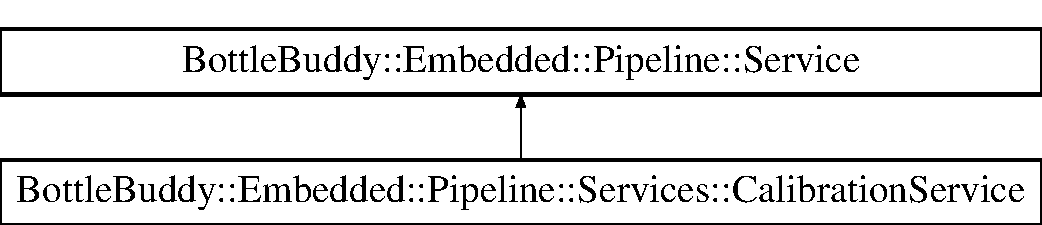
\includegraphics[height=2.000000cm]{class_bottle_buddy_1_1_embedded_1_1_pipeline_1_1_services_1_1_calibration_service}
\end{center}
\end{figure}
\subsection*{Public Member Functions}
\begin{DoxyCompactItemize}
\item 
{\bfseries Calibration\+Service} (const char $\ast$\hyperlink{class_bottle_buddy_1_1_embedded_1_1_pipeline_1_1_service_af290f9aa0a6dca36e802e615fab19f78}{uid})\hypertarget{class_bottle_buddy_1_1_embedded_1_1_pipeline_1_1_services_1_1_calibration_service_a5026856c587f00b3d81b71dda1a07328}{}\label{class_bottle_buddy_1_1_embedded_1_1_pipeline_1_1_services_1_1_calibration_service_a5026856c587f00b3d81b71dda1a07328}

\item 
void {\bfseries connect} (B\+L\+E\+Device central)\hypertarget{class_bottle_buddy_1_1_embedded_1_1_pipeline_1_1_services_1_1_calibration_service_a03120337e0f8d93dce193acc6bca1864}{}\label{class_bottle_buddy_1_1_embedded_1_1_pipeline_1_1_services_1_1_calibration_service_a03120337e0f8d93dce193acc6bca1864}

\item 
void {\bfseries disconnect} (B\+L\+E\+Device central)\hypertarget{class_bottle_buddy_1_1_embedded_1_1_pipeline_1_1_services_1_1_calibration_service_aa6e97a614358122ae479064f2dfc0608}{}\label{class_bottle_buddy_1_1_embedded_1_1_pipeline_1_1_services_1_1_calibration_service_aa6e97a614358122ae479064f2dfc0608}

\item 
void {\bfseries loop} ()\hypertarget{class_bottle_buddy_1_1_embedded_1_1_pipeline_1_1_services_1_1_calibration_service_a63f4a7194f070f9f87b2ec6918caabd8}{}\label{class_bottle_buddy_1_1_embedded_1_1_pipeline_1_1_services_1_1_calibration_service_a63f4a7194f070f9f87b2ec6918caabd8}

\item 
void \hyperlink{class_bottle_buddy_1_1_embedded_1_1_pipeline_1_1_services_1_1_calibration_service_aa1eef705812548b2251bbe08e1a07933}{receive} (\hyperlink{class_bottle_buddy_1_1_embedded_1_1_pipeline_1_1_package}{Package} $\ast$package)
\begin{DoxyCompactList}\small\item\em Used by the router class to deliver a package to a service. \end{DoxyCompactList}\item 
bool {\bfseries calibrated\+Bottle\+Buddy} ()\hypertarget{class_bottle_buddy_1_1_embedded_1_1_pipeline_1_1_services_1_1_calibration_service_a7981aa9664dc6a236f52ddb0edacdc21}{}\label{class_bottle_buddy_1_1_embedded_1_1_pipeline_1_1_services_1_1_calibration_service_a7981aa9664dc6a236f52ddb0edacdc21}

\item 
unsigned int {\bfseries get\+Date} ()\hypertarget{class_bottle_buddy_1_1_embedded_1_1_pipeline_1_1_services_1_1_calibration_service_a9c12bcefd34b1e5e1d7ab8d5c1e7aaac}{}\label{class_bottle_buddy_1_1_embedded_1_1_pipeline_1_1_services_1_1_calibration_service_a9c12bcefd34b1e5e1d7ab8d5c1e7aaac}

\item 
unsigned int {\bfseries get\+Time} ()\hypertarget{class_bottle_buddy_1_1_embedded_1_1_pipeline_1_1_services_1_1_calibration_service_a2758feaa416436d7d271ff2f3dbc9555}{}\label{class_bottle_buddy_1_1_embedded_1_1_pipeline_1_1_services_1_1_calibration_service_a2758feaa416436d7d271ff2f3dbc9555}

\end{DoxyCompactItemize}
\subsection*{Additional Inherited Members}


\subsection{Member Function Documentation}
\index{Bottle\+Buddy\+::\+Embedded\+::\+Pipeline\+::\+Services\+::\+Calibration\+Service@{Bottle\+Buddy\+::\+Embedded\+::\+Pipeline\+::\+Services\+::\+Calibration\+Service}!receive@{receive}}
\index{receive@{receive}!Bottle\+Buddy\+::\+Embedded\+::\+Pipeline\+::\+Services\+::\+Calibration\+Service@{Bottle\+Buddy\+::\+Embedded\+::\+Pipeline\+::\+Services\+::\+Calibration\+Service}}
\subsubsection[{\texorpdfstring{receive(\+Package $\ast$package)}{receive(Package *package)}}]{\setlength{\rightskip}{0pt plus 5cm}void Bottle\+Buddy\+::\+Embedded\+::\+Pipeline\+::\+Services\+::\+Calibration\+Service\+::receive (
\begin{DoxyParamCaption}
\item[{{\bf Package} $\ast$}]{package}
\end{DoxyParamCaption}
)\hspace{0.3cm}{\ttfamily [virtual]}}\hypertarget{class_bottle_buddy_1_1_embedded_1_1_pipeline_1_1_services_1_1_calibration_service_aa1eef705812548b2251bbe08e1a07933}{}\label{class_bottle_buddy_1_1_embedded_1_1_pipeline_1_1_services_1_1_calibration_service_aa1eef705812548b2251bbe08e1a07933}


Used by the router class to deliver a package to a service. 

Can be implemented however the derived service needs in order to provide its service. 

Implements \hyperlink{class_bottle_buddy_1_1_embedded_1_1_pipeline_1_1_service_aaa0ee18450e47f2ad51d9934a2d61992}{Bottle\+Buddy\+::\+Embedded\+::\+Pipeline\+::\+Service}.



The documentation for this class was generated from the following files\+:\begin{DoxyCompactItemize}
\item 
/home/travis/build/\+Bottle\+Buddy/bottle-\/buddy-\/embedded/include/\+Pipeline/\+Services/\hyperlink{calibration_service_8h}{calibration\+Service.\+h}\item 
/home/travis/build/\+Bottle\+Buddy/bottle-\/buddy-\/embedded/src/\+Pipeline/\+Services/\hyperlink{calibration_service_8cpp}{calibration\+Service.\+cpp}\end{DoxyCompactItemize}

\hypertarget{class_bottle_buddy_1_1_embedded_1_1_pipeline_1_1_services_1_1_cleaning_service}{}\section{Bottle\+Buddy\+:\+:Embedded\+:\+:Pipeline\+:\+:Services\+:\+:Cleaning\+Service Class Reference}
\label{class_bottle_buddy_1_1_embedded_1_1_pipeline_1_1_services_1_1_cleaning_service}\index{Bottle\+Buddy\+::\+Embedded\+::\+Pipeline\+::\+Services\+::\+Cleaning\+Service@{Bottle\+Buddy\+::\+Embedded\+::\+Pipeline\+::\+Services\+::\+Cleaning\+Service}}


This class automatically cleans the users bottle.  




{\ttfamily \#include $<$cleaning\+Service.\+h$>$}

Inheritance diagram for Bottle\+Buddy\+:\+:Embedded\+:\+:Pipeline\+:\+:Services\+:\+:Cleaning\+Service\+:\begin{figure}[H]
\begin{center}
\leavevmode
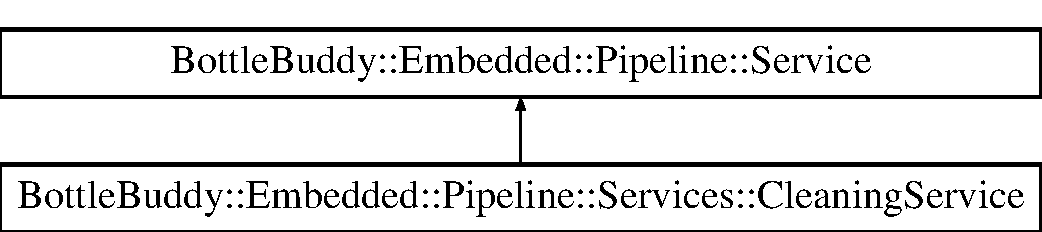
\includegraphics[height=2.000000cm]{class_bottle_buddy_1_1_embedded_1_1_pipeline_1_1_services_1_1_cleaning_service}
\end{center}
\end{figure}
\subsection*{Public Member Functions}
\begin{DoxyCompactItemize}
\item 
{\bfseries Cleaning\+Service} (const char $\ast$\hyperlink{class_bottle_buddy_1_1_embedded_1_1_pipeline_1_1_service_af290f9aa0a6dca36e802e615fab19f78}{uid}, bool connected=false)\hypertarget{class_bottle_buddy_1_1_embedded_1_1_pipeline_1_1_services_1_1_cleaning_service_ae9c3e69b06b31505540b274e8f00cf9d}{}\label{class_bottle_buddy_1_1_embedded_1_1_pipeline_1_1_services_1_1_cleaning_service_ae9c3e69b06b31505540b274e8f00cf9d}

\item 
void {\bfseries connect} (B\+L\+E\+Device central)\hypertarget{class_bottle_buddy_1_1_embedded_1_1_pipeline_1_1_services_1_1_cleaning_service_aed7ca1580dbfadaa0f009283df62cd5d}{}\label{class_bottle_buddy_1_1_embedded_1_1_pipeline_1_1_services_1_1_cleaning_service_aed7ca1580dbfadaa0f009283df62cd5d}

\item 
void {\bfseries disconnect} (B\+L\+E\+Device central)\hypertarget{class_bottle_buddy_1_1_embedded_1_1_pipeline_1_1_services_1_1_cleaning_service_aa3588e480fd6aa5d19e0cb78826798d9}{}\label{class_bottle_buddy_1_1_embedded_1_1_pipeline_1_1_services_1_1_cleaning_service_aa3588e480fd6aa5d19e0cb78826798d9}

\item 
void {\bfseries loop} ()\hypertarget{class_bottle_buddy_1_1_embedded_1_1_pipeline_1_1_services_1_1_cleaning_service_a86e7fd7dfa11b12b7d10463a232f105e}{}\label{class_bottle_buddy_1_1_embedded_1_1_pipeline_1_1_services_1_1_cleaning_service_a86e7fd7dfa11b12b7d10463a232f105e}

\item 
void \hyperlink{class_bottle_buddy_1_1_embedded_1_1_pipeline_1_1_services_1_1_cleaning_service_a6d3dee7ca6387c00cec3478821b1ea23}{receive} (\hyperlink{class_bottle_buddy_1_1_embedded_1_1_pipeline_1_1_package}{Package} $\ast$package)
\begin{DoxyCompactList}\small\item\em Used by the router class to deliver a package to a service. \end{DoxyCompactList}\end{DoxyCompactItemize}
\subsection*{Static Public Member Functions}
\begin{DoxyCompactItemize}
\item 
static bool \hyperlink{class_bottle_buddy_1_1_embedded_1_1_pipeline_1_1_services_1_1_cleaning_service_a122a4f47c702c950ed601050e5be9242}{finish\+Cleaning} (void $\ast$cleaning\+Instance)
\begin{DoxyCompactList}\small\item\em Called when cleaning successfully completes. \end{DoxyCompactList}\end{DoxyCompactItemize}
\subsection*{Additional Inherited Members}


\subsection{Detailed Description}
This class automatically cleans the users bottle. 

When the Bottle Buddy app determines that the user\textquotesingle{}s bottle is due for a cleaning session, this class will receive that information then initiate cleaning once it has determined it is safe. 

\subsection{Member Function Documentation}
\index{Bottle\+Buddy\+::\+Embedded\+::\+Pipeline\+::\+Services\+::\+Cleaning\+Service@{Bottle\+Buddy\+::\+Embedded\+::\+Pipeline\+::\+Services\+::\+Cleaning\+Service}!finish\+Cleaning@{finish\+Cleaning}}
\index{finish\+Cleaning@{finish\+Cleaning}!Bottle\+Buddy\+::\+Embedded\+::\+Pipeline\+::\+Services\+::\+Cleaning\+Service@{Bottle\+Buddy\+::\+Embedded\+::\+Pipeline\+::\+Services\+::\+Cleaning\+Service}}
\subsubsection[{\texorpdfstring{finish\+Cleaning(void $\ast$cleaning\+Instance)}{finishCleaning(void *cleaningInstance)}}]{\setlength{\rightskip}{0pt plus 5cm}bool Bottle\+Buddy\+::\+Embedded\+::\+Pipeline\+::\+Services\+::\+Cleaning\+Service\+::finish\+Cleaning (
\begin{DoxyParamCaption}
\item[{void $\ast$}]{cleaning\+Instance}
\end{DoxyParamCaption}
)\hspace{0.3cm}{\ttfamily [static]}}\hypertarget{class_bottle_buddy_1_1_embedded_1_1_pipeline_1_1_services_1_1_cleaning_service_a122a4f47c702c950ed601050e5be9242}{}\label{class_bottle_buddy_1_1_embedded_1_1_pipeline_1_1_services_1_1_cleaning_service_a122a4f47c702c950ed601050e5be9242}


Called when cleaning successfully completes. 

Once the cap is on for at least 10 seconds after the app initiates cleaning, this function turns the U\+VC light off and notifies the app. \index{Bottle\+Buddy\+::\+Embedded\+::\+Pipeline\+::\+Services\+::\+Cleaning\+Service@{Bottle\+Buddy\+::\+Embedded\+::\+Pipeline\+::\+Services\+::\+Cleaning\+Service}!receive@{receive}}
\index{receive@{receive}!Bottle\+Buddy\+::\+Embedded\+::\+Pipeline\+::\+Services\+::\+Cleaning\+Service@{Bottle\+Buddy\+::\+Embedded\+::\+Pipeline\+::\+Services\+::\+Cleaning\+Service}}
\subsubsection[{\texorpdfstring{receive(\+Package $\ast$package)}{receive(Package *package)}}]{\setlength{\rightskip}{0pt plus 5cm}void Bottle\+Buddy\+::\+Embedded\+::\+Pipeline\+::\+Services\+::\+Cleaning\+Service\+::receive (
\begin{DoxyParamCaption}
\item[{{\bf Package} $\ast$}]{package}
\end{DoxyParamCaption}
)\hspace{0.3cm}{\ttfamily [virtual]}}\hypertarget{class_bottle_buddy_1_1_embedded_1_1_pipeline_1_1_services_1_1_cleaning_service_a6d3dee7ca6387c00cec3478821b1ea23}{}\label{class_bottle_buddy_1_1_embedded_1_1_pipeline_1_1_services_1_1_cleaning_service_a6d3dee7ca6387c00cec3478821b1ea23}


Used by the router class to deliver a package to a service. 

Can be implemented however the derived service needs in order to provide its service. 

Implements \hyperlink{class_bottle_buddy_1_1_embedded_1_1_pipeline_1_1_service_aaa0ee18450e47f2ad51d9934a2d61992}{Bottle\+Buddy\+::\+Embedded\+::\+Pipeline\+::\+Service}.



The documentation for this class was generated from the following files\+:\begin{DoxyCompactItemize}
\item 
/home/travis/build/\+Bottle\+Buddy/bottle-\/buddy-\/embedded/include/\+Pipeline/\+Services/\hyperlink{cleaning_service_8h}{cleaning\+Service.\+h}\item 
/home/travis/build/\+Bottle\+Buddy/bottle-\/buddy-\/embedded/src/\+Pipeline/\+Services/\hyperlink{cleaning_service_8cpp}{cleaning\+Service.\+cpp}\end{DoxyCompactItemize}

\hypertarget{class_bottle_buddy_1_1_embedded_1_1_pipeline_1_1_package}{}\section{Bottle\+Buddy\+:\+:Embedded\+:\+:Pipeline\+:\+:Package Class Reference}
\label{class_bottle_buddy_1_1_embedded_1_1_pipeline_1_1_package}\index{Bottle\+Buddy\+::\+Embedded\+::\+Pipeline\+::\+Package@{Bottle\+Buddy\+::\+Embedded\+::\+Pipeline\+::\+Package}}


Encapsulates low level sensor data traveling through the pipeline.  




{\ttfamily \#include $<$package.\+h$>$}

\subsection*{Public Member Functions}
\begin{DoxyCompactItemize}
\item 
{\bfseries Package} (\hyperlink{package_8h_aea2eca0caf9ed97414998f1a2f404682}{Location} origin, int data)\hypertarget{class_bottle_buddy_1_1_embedded_1_1_pipeline_1_1_package_adf8ec5ae75a12391187e5b75b6b048cd}{}\label{class_bottle_buddy_1_1_embedded_1_1_pipeline_1_1_package_adf8ec5ae75a12391187e5b75b6b048cd}

\item 
{\bfseries Package} (\hyperlink{package_8h_aea2eca0caf9ed97414998f1a2f404682}{Location} origin, float data)\hypertarget{class_bottle_buddy_1_1_embedded_1_1_pipeline_1_1_package_ad18d73be8fdfba561482fac9294a3ab5}{}\label{class_bottle_buddy_1_1_embedded_1_1_pipeline_1_1_package_ad18d73be8fdfba561482fac9294a3ab5}

\item 
{\bfseries Package} (\hyperlink{package_8h_aea2eca0caf9ed97414998f1a2f404682}{Location} origin, int dim1, int dim2)\hypertarget{class_bottle_buddy_1_1_embedded_1_1_pipeline_1_1_package_a4413e84509500a4c31dfabd2ab580003}{}\label{class_bottle_buddy_1_1_embedded_1_1_pipeline_1_1_package_a4413e84509500a4c31dfabd2ab580003}

\item 
{\bfseries Package} (\hyperlink{package_8h_aea2eca0caf9ed97414998f1a2f404682}{Location} origin, float dim1, float dim2)\hypertarget{class_bottle_buddy_1_1_embedded_1_1_pipeline_1_1_package_a740d736bbc74a8bdb5d5b164449fa534}{}\label{class_bottle_buddy_1_1_embedded_1_1_pipeline_1_1_package_a740d736bbc74a8bdb5d5b164449fa534}

\item 
{\bfseries Package} (\hyperlink{package_8h_aea2eca0caf9ed97414998f1a2f404682}{Location} origin, int dim1, int dim2, int dim3)\hypertarget{class_bottle_buddy_1_1_embedded_1_1_pipeline_1_1_package_a71028ce733f073b9477c17cae72720ed}{}\label{class_bottle_buddy_1_1_embedded_1_1_pipeline_1_1_package_a71028ce733f073b9477c17cae72720ed}

\item 
{\bfseries Package} (\hyperlink{package_8h_aea2eca0caf9ed97414998f1a2f404682}{Location} origin, float dim1, float dim2, float dim3)\hypertarget{class_bottle_buddy_1_1_embedded_1_1_pipeline_1_1_package_aa49bd59f49c6834ae5b3993c28bdb77e}{}\label{class_bottle_buddy_1_1_embedded_1_1_pipeline_1_1_package_aa49bd59f49c6834ae5b3993c28bdb77e}

\item 
\hyperlink{package_8h_aea2eca0caf9ed97414998f1a2f404682}{Location} \hyperlink{class_bottle_buddy_1_1_embedded_1_1_pipeline_1_1_package_a66721d7273ffb4535d3a98e24ea26099}{get\+Origin} ()\hypertarget{class_bottle_buddy_1_1_embedded_1_1_pipeline_1_1_package_a66721d7273ffb4535d3a98e24ea26099}{}\label{class_bottle_buddy_1_1_embedded_1_1_pipeline_1_1_package_a66721d7273ffb4535d3a98e24ea26099}

\begin{DoxyCompactList}\small\item\em Returns the location corresponding to which sensor this package is from. \end{DoxyCompactList}\item 
bool {\bfseries get\+Data} (int \&data)\hypertarget{class_bottle_buddy_1_1_embedded_1_1_pipeline_1_1_package_a6dddf8a0ef79d947a4cef0b2e349af6b}{}\label{class_bottle_buddy_1_1_embedded_1_1_pipeline_1_1_package_a6dddf8a0ef79d947a4cef0b2e349af6b}

\item 
bool {\bfseries get\+Data} (int \&dim1, int \&dim2)\hypertarget{class_bottle_buddy_1_1_embedded_1_1_pipeline_1_1_package_a6ad1e786cdc50c7582dc26b3157ae593}{}\label{class_bottle_buddy_1_1_embedded_1_1_pipeline_1_1_package_a6ad1e786cdc50c7582dc26b3157ae593}

\item 
bool {\bfseries get\+Data} (int \&dim1, int \&dim2, int \&dim3)\hypertarget{class_bottle_buddy_1_1_embedded_1_1_pipeline_1_1_package_a977cec6790ace8b8fa4c7d9615ba0c76}{}\label{class_bottle_buddy_1_1_embedded_1_1_pipeline_1_1_package_a977cec6790ace8b8fa4c7d9615ba0c76}

\item 
bool {\bfseries get\+Data} (float \&data)\hypertarget{class_bottle_buddy_1_1_embedded_1_1_pipeline_1_1_package_a81c5856398146b39b1223f0e2644efd5}{}\label{class_bottle_buddy_1_1_embedded_1_1_pipeline_1_1_package_a81c5856398146b39b1223f0e2644efd5}

\item 
bool {\bfseries get\+Data} (float \&dim1, float \&dim2)\hypertarget{class_bottle_buddy_1_1_embedded_1_1_pipeline_1_1_package_afa39a20f1a710af1fd7ccf20b9883be4}{}\label{class_bottle_buddy_1_1_embedded_1_1_pipeline_1_1_package_afa39a20f1a710af1fd7ccf20b9883be4}

\item 
bool {\bfseries get\+Data} (float \&dim1, float \&dim2, float \&dim3)\hypertarget{class_bottle_buddy_1_1_embedded_1_1_pipeline_1_1_package_ae42a459cd0780733c9d4700814a26672}{}\label{class_bottle_buddy_1_1_embedded_1_1_pipeline_1_1_package_ae42a459cd0780733c9d4700814a26672}

\end{DoxyCompactItemize}


\subsection{Detailed Description}
Encapsulates low level sensor data traveling through the pipeline. 

This class provides a clean interface both for low level drives to transport their sensor data as well as high level services to read data from low level sensors. 

The documentation for this class was generated from the following files\+:\begin{DoxyCompactItemize}
\item 
/home/travis/build/\+Bottle\+Buddy/bottle-\/buddy-\/embedded/include/\+Pipeline/\hyperlink{package_8h}{package.\+h}\item 
/home/travis/build/\+Bottle\+Buddy/bottle-\/buddy-\/embedded/src/\+Pipeline/\hyperlink{package_8cpp}{package.\+cpp}\end{DoxyCompactItemize}

\hypertarget{struct_bottle_buddy_1_1_embedded_1_1_pipeline_1_1_pending_service}{}\section{Bottle\+Buddy\+:\+:Embedded\+:\+:Pipeline\+:\+:Pending\+Service Struct Reference}
\label{struct_bottle_buddy_1_1_embedded_1_1_pipeline_1_1_pending_service}\index{Bottle\+Buddy\+::\+Embedded\+::\+Pipeline\+::\+Pending\+Service@{Bottle\+Buddy\+::\+Embedded\+::\+Pipeline\+::\+Pending\+Service}}
\subsection*{Public Attributes}
\begin{DoxyCompactItemize}
\item 
Service\+Type {\bfseries service\+Type}\hypertarget{struct_bottle_buddy_1_1_embedded_1_1_pipeline_1_1_pending_service_aebbf3dc0ea2ca5a53d8a14620b11b157}{}\label{struct_bottle_buddy_1_1_embedded_1_1_pipeline_1_1_pending_service_aebbf3dc0ea2ca5a53d8a14620b11b157}

\item 
const char $\ast$ {\bfseries uid}\hypertarget{struct_bottle_buddy_1_1_embedded_1_1_pipeline_1_1_pending_service_a1df5c11180f83e1a27eceabd439e2000}{}\label{struct_bottle_buddy_1_1_embedded_1_1_pipeline_1_1_pending_service_a1df5c11180f83e1a27eceabd439e2000}

\end{DoxyCompactItemize}


The documentation for this struct was generated from the following file\+:\begin{DoxyCompactItemize}
\item 
/home/travis/build/\+Bottle\+Buddy/bottle-\/buddy-\/embedded/include/\+Pipeline/\hyperlink{service_manager_8h}{service\+Manager.\+h}\end{DoxyCompactItemize}

\hypertarget{class_bottle_buddy_1_1_embedded_1_1_pipeline_1_1_pipe}{}\section{Bottle\+Buddy\+:\+:Embedded\+:\+:Pipeline\+:\+:Pipe Class Reference}
\label{class_bottle_buddy_1_1_embedded_1_1_pipeline_1_1_pipe}\index{Bottle\+Buddy\+::\+Embedded\+::\+Pipeline\+::\+Pipe@{Bottle\+Buddy\+::\+Embedded\+::\+Pipeline\+::\+Pipe}}


Transports sensor data.  




{\ttfamily \#include $<$pipe.\+h$>$}

\subsection*{Public Member Functions}
\begin{DoxyCompactItemize}
\item 
{\bfseries Pipe} (\hyperlink{package_8h_aea2eca0caf9ed97414998f1a2f404682}{Location} location)\hypertarget{class_bottle_buddy_1_1_embedded_1_1_pipeline_1_1_pipe_a74724b71f6b5c7860c0111040b548244}{}\label{class_bottle_buddy_1_1_embedded_1_1_pipeline_1_1_pipe_a74724b71f6b5c7860c0111040b548244}

\item 
{\footnotesize template$<$typename T $>$ }\\void \hyperlink{class_bottle_buddy_1_1_embedded_1_1_pipeline_1_1_pipe_a4f344a817c439a96e28d1a226de4054b}{send\+Payload} (T data)
\begin{DoxyCompactList}\small\item\em Sends sensor data. \end{DoxyCompactList}\item 
{\footnotesize template$<$typename T $>$ }\\void {\bfseries send\+Payload} (T dim1, T dim2)\hypertarget{class_bottle_buddy_1_1_embedded_1_1_pipeline_1_1_pipe_a8007c53c651b37348f010c879e8ca42a}{}\label{class_bottle_buddy_1_1_embedded_1_1_pipeline_1_1_pipe_a8007c53c651b37348f010c879e8ca42a}

\item 
{\footnotesize template$<$typename T $>$ }\\void {\bfseries send\+Payload} (T dim1, T dim2, T dim3)\hypertarget{class_bottle_buddy_1_1_embedded_1_1_pipeline_1_1_pipe_a8f670b3591991a5afbae53d4ab5bc202}{}\label{class_bottle_buddy_1_1_embedded_1_1_pipeline_1_1_pipe_a8f670b3591991a5afbae53d4ab5bc202}

\end{DoxyCompactItemize}


\subsection{Detailed Description}
Transports sensor data. 

This is a general class used to bi-\/directionally transport sensor data across the Bottle Buddy embedded system. 

\subsection{Member Function Documentation}
\index{Bottle\+Buddy\+::\+Embedded\+::\+Pipeline\+::\+Pipe@{Bottle\+Buddy\+::\+Embedded\+::\+Pipeline\+::\+Pipe}!send\+Payload@{send\+Payload}}
\index{send\+Payload@{send\+Payload}!Bottle\+Buddy\+::\+Embedded\+::\+Pipeline\+::\+Pipe@{Bottle\+Buddy\+::\+Embedded\+::\+Pipeline\+::\+Pipe}}
\subsubsection[{\texorpdfstring{send\+Payload(\+T data)}{sendPayload(T data)}}]{\setlength{\rightskip}{0pt plus 5cm}template$<$typename T $>$ void Bottle\+Buddy\+::\+Embedded\+::\+Pipeline\+::\+Pipe\+::send\+Payload (
\begin{DoxyParamCaption}
\item[{T}]{data}
\end{DoxyParamCaption}
)}\hypertarget{class_bottle_buddy_1_1_embedded_1_1_pipeline_1_1_pipe_a4f344a817c439a96e28d1a226de4054b}{}\label{class_bottle_buddy_1_1_embedded_1_1_pipeline_1_1_pipe_a4f344a817c439a96e28d1a226de4054b}


Sends sensor data. 

Use this function when a sensor reads new data that will be used across the Bottle Buddy embedded system. 

The documentation for this class was generated from the following files\+:\begin{DoxyCompactItemize}
\item 
/home/travis/build/\+Bottle\+Buddy/bottle-\/buddy-\/embedded/include/\+Pipeline/\hyperlink{pipe_8h}{pipe.\+h}\item 
/home/travis/build/\+Bottle\+Buddy/bottle-\/buddy-\/embedded/src/\+Pipeline/\hyperlink{pipe_8cpp}{pipe.\+cpp}\end{DoxyCompactItemize}

\hypertarget{class_bottle_buddy_1_1_embedded_1_1_pipeline_1_1_router}{}\section{Bottle\+Buddy\+:\+:Embedded\+:\+:Pipeline\+:\+:Router Class Reference}
\label{class_bottle_buddy_1_1_embedded_1_1_pipeline_1_1_router}\index{Bottle\+Buddy\+::\+Embedded\+::\+Pipeline\+::\+Router@{Bottle\+Buddy\+::\+Embedded\+::\+Pipeline\+::\+Router}}


Handles package delivery.  




{\ttfamily \#include $<$router.\+h$>$}

\subsection*{Static Public Member Functions}
\begin{DoxyCompactItemize}
\item 
static void \hyperlink{class_bottle_buddy_1_1_embedded_1_1_pipeline_1_1_router_a9a56d0c05698c1ee0ad398fc87832a6c}{route} (\hyperlink{class_bottle_buddy_1_1_embedded_1_1_pipeline_1_1_package}{Package} $\ast$package)
\begin{DoxyCompactList}\small\item\em Routes packages coming from a pipe. \end{DoxyCompactList}\item 
static void \hyperlink{class_bottle_buddy_1_1_embedded_1_1_pipeline_1_1_router_a49274f0fc1baa9823f645bfabbbb137a}{subscribe} (\hyperlink{package_8h_aea2eca0caf9ed97414998f1a2f404682}{Location} location, \hyperlink{class_bottle_buddy_1_1_embedded_1_1_pipeline_1_1_service}{Service} $\ast$service)
\begin{DoxyCompactList}\small\item\em Subscribes a service to a sensor location. \end{DoxyCompactList}\end{DoxyCompactItemize}


\subsection{Detailed Description}
Handles package delivery. 

\subsection{Member Function Documentation}
\index{Bottle\+Buddy\+::\+Embedded\+::\+Pipeline\+::\+Router@{Bottle\+Buddy\+::\+Embedded\+::\+Pipeline\+::\+Router}!route@{route}}
\index{route@{route}!Bottle\+Buddy\+::\+Embedded\+::\+Pipeline\+::\+Router@{Bottle\+Buddy\+::\+Embedded\+::\+Pipeline\+::\+Router}}
\subsubsection[{\texorpdfstring{route(\+Package $\ast$package)}{route(Package *package)}}]{\setlength{\rightskip}{0pt plus 5cm}void Bottle\+Buddy\+::\+Embedded\+::\+Pipeline\+::\+Router\+::route (
\begin{DoxyParamCaption}
\item[{{\bf Package} $\ast$}]{package}
\end{DoxyParamCaption}
)\hspace{0.3cm}{\ttfamily [static]}}\hypertarget{class_bottle_buddy_1_1_embedded_1_1_pipeline_1_1_router_a9a56d0c05698c1ee0ad398fc87832a6c}{}\label{class_bottle_buddy_1_1_embedded_1_1_pipeline_1_1_router_a9a56d0c05698c1ee0ad398fc87832a6c}


Routes packages coming from a pipe. 

Route\textquotesingle{}s a pipe\textquotesingle{}s package to every service subscribed to that location. \index{Bottle\+Buddy\+::\+Embedded\+::\+Pipeline\+::\+Router@{Bottle\+Buddy\+::\+Embedded\+::\+Pipeline\+::\+Router}!subscribe@{subscribe}}
\index{subscribe@{subscribe}!Bottle\+Buddy\+::\+Embedded\+::\+Pipeline\+::\+Router@{Bottle\+Buddy\+::\+Embedded\+::\+Pipeline\+::\+Router}}
\subsubsection[{\texorpdfstring{subscribe(\+Location location, Service $\ast$service)}{subscribe(Location location, Service *service)}}]{\setlength{\rightskip}{0pt plus 5cm}void Bottle\+Buddy\+::\+Embedded\+::\+Pipeline\+::\+Router\+::subscribe (
\begin{DoxyParamCaption}
\item[{{\bf Location}}]{location, }
\item[{{\bf Service} $\ast$}]{service}
\end{DoxyParamCaption}
)\hspace{0.3cm}{\ttfamily [static]}}\hypertarget{class_bottle_buddy_1_1_embedded_1_1_pipeline_1_1_router_a49274f0fc1baa9823f645bfabbbb137a}{}\label{class_bottle_buddy_1_1_embedded_1_1_pipeline_1_1_router_a49274f0fc1baa9823f645bfabbbb137a}


Subscribes a service to a sensor location. 

If a service needs a specific sensor\textquotesingle{}s data to provide its service, then calling this function will allow the service specified to begin receiving data from the location specified. 

The documentation for this class was generated from the following files\+:\begin{DoxyCompactItemize}
\item 
/home/travis/build/\+Bottle\+Buddy/bottle-\/buddy-\/embedded/include/\+Pipeline/\hyperlink{router_8h}{router.\+h}\item 
/home/travis/build/\+Bottle\+Buddy/bottle-\/buddy-\/embedded/src/\+Pipeline/\hyperlink{router_8cpp}{router.\+cpp}\end{DoxyCompactItemize}

\hypertarget{class_bottle_buddy_1_1_embedded_1_1_pipeline_1_1_service}{}\section{Bottle\+Buddy\+:\+:Embedded\+:\+:Pipeline\+:\+:Service Class Reference}
\label{class_bottle_buddy_1_1_embedded_1_1_pipeline_1_1_service}\index{Bottle\+Buddy\+::\+Embedded\+::\+Pipeline\+::\+Service@{Bottle\+Buddy\+::\+Embedded\+::\+Pipeline\+::\+Service}}


Base class for high level services.  




{\ttfamily \#include $<$service.\+h$>$}

Inheritance diagram for Bottle\+Buddy\+:\+:Embedded\+:\+:Pipeline\+:\+:Service\+:\begin{figure}[H]
\begin{center}
\leavevmode
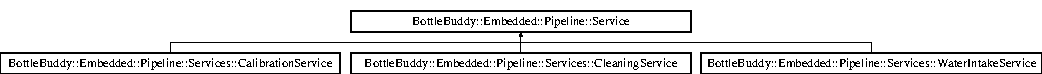
\includegraphics[height=0.995556cm]{class_bottle_buddy_1_1_embedded_1_1_pipeline_1_1_service}
\end{center}
\end{figure}
\subsection*{Public Member Functions}
\begin{DoxyCompactItemize}
\item 
{\bfseries Service} (const char $\ast$\hyperlink{class_bottle_buddy_1_1_embedded_1_1_pipeline_1_1_service_af290f9aa0a6dca36e802e615fab19f78}{uid}, bool connected=false)\hypertarget{class_bottle_buddy_1_1_embedded_1_1_pipeline_1_1_service_a8381de83d01e2c167746b1c8bc698552}{}\label{class_bottle_buddy_1_1_embedded_1_1_pipeline_1_1_service_a8381de83d01e2c167746b1c8bc698552}

\item 
virtual void {\bfseries connect} (B\+L\+E\+Device central)=0\hypertarget{class_bottle_buddy_1_1_embedded_1_1_pipeline_1_1_service_a9255768adea0f606df15d4e991bc88cf}{}\label{class_bottle_buddy_1_1_embedded_1_1_pipeline_1_1_service_a9255768adea0f606df15d4e991bc88cf}

\item 
virtual void {\bfseries disconnect} (B\+L\+E\+Device central)=0\hypertarget{class_bottle_buddy_1_1_embedded_1_1_pipeline_1_1_service_a151d906c9cbbac783c74fb6c8f17ffcc}{}\label{class_bottle_buddy_1_1_embedded_1_1_pipeline_1_1_service_a151d906c9cbbac783c74fb6c8f17ffcc}

\item 
virtual void {\bfseries loop} ()=0\hypertarget{class_bottle_buddy_1_1_embedded_1_1_pipeline_1_1_service_ab2e3087822ea3768ce176b64b43ec706}{}\label{class_bottle_buddy_1_1_embedded_1_1_pipeline_1_1_service_ab2e3087822ea3768ce176b64b43ec706}

\item 
virtual void \hyperlink{class_bottle_buddy_1_1_embedded_1_1_pipeline_1_1_service_aaa0ee18450e47f2ad51d9934a2d61992}{receive} (\hyperlink{class_bottle_buddy_1_1_embedded_1_1_pipeline_1_1_package}{Package} $\ast$package)=0
\begin{DoxyCompactList}\small\item\em Used by the router class to deliver a package to a service. \end{DoxyCompactList}\end{DoxyCompactItemize}
\subsection*{Protected Member Functions}
\begin{DoxyCompactItemize}
\item 
bool \hyperlink{class_bottle_buddy_1_1_embedded_1_1_pipeline_1_1_service_a7883b3a53fc8e6f9d457d7d164853c37}{create\+Characteristic} (std\+::string name, uint8\+\_\+t properties, B\+L\+E\+Type characteristic\+Type)
\begin{DoxyCompactList}\small\item\em Used to create a new characteristics within the B\+LE module. \end{DoxyCompactList}\item 
B\+L\+E\+Characteristic $\ast$ {\bfseries get\+Characteristic} (std\+::string name)\hypertarget{class_bottle_buddy_1_1_embedded_1_1_pipeline_1_1_service_a3dbda00416a45e1e5d0a8652fd126768}{}\label{class_bottle_buddy_1_1_embedded_1_1_pipeline_1_1_service_a3dbda00416a45e1e5d0a8652fd126768}

\item 
B\+L\+E\+String\+Characteristic $\ast$ {\bfseries get\+String\+Characteristic} (std\+::string name)\hypertarget{class_bottle_buddy_1_1_embedded_1_1_pipeline_1_1_service_ab5c898cc7b6ebde52a8205579890a105}{}\label{class_bottle_buddy_1_1_embedded_1_1_pipeline_1_1_service_ab5c898cc7b6ebde52a8205579890a105}

\end{DoxyCompactItemize}
\subsection*{Protected Attributes}
\begin{DoxyCompactItemize}
\item 
const char $\ast$ \hyperlink{class_bottle_buddy_1_1_embedded_1_1_pipeline_1_1_service_af290f9aa0a6dca36e802e615fab19f78}{uid}\hypertarget{class_bottle_buddy_1_1_embedded_1_1_pipeline_1_1_service_af290f9aa0a6dca36e802e615fab19f78}{}\label{class_bottle_buddy_1_1_embedded_1_1_pipeline_1_1_service_af290f9aa0a6dca36e802e615fab19f78}

\begin{DoxyCompactList}\small\item\em The service\textquotesingle{}s U\+ID string, which is used for B\+LE purposes. \end{DoxyCompactList}\item 
B\+L\+E\+Service $\ast$ \hyperlink{class_bottle_buddy_1_1_embedded_1_1_pipeline_1_1_service_a630b006fa103113e214455827c5f0b9b}{ble\+Service}\hypertarget{class_bottle_buddy_1_1_embedded_1_1_pipeline_1_1_service_a630b006fa103113e214455827c5f0b9b}{}\label{class_bottle_buddy_1_1_embedded_1_1_pipeline_1_1_service_a630b006fa103113e214455827c5f0b9b}

\begin{DoxyCompactList}\small\item\em The services B\+L\+E\+Service variable, which creates a new service within the B\+LE module. \end{DoxyCompactList}\item 
bool {\bfseries connected}\hypertarget{class_bottle_buddy_1_1_embedded_1_1_pipeline_1_1_service_a04c95502999a9d66577a016ba2bf39c7}{}\label{class_bottle_buddy_1_1_embedded_1_1_pipeline_1_1_service_a04c95502999a9d66577a016ba2bf39c7}

\item 
std\+::vector$<$ const char $\ast$ $>$ \hyperlink{class_bottle_buddy_1_1_embedded_1_1_pipeline_1_1_service_a543fc4a07564a076ffc2835510763e5f}{uuids}
\begin{DoxyCompactList}\small\item\em Vector of characteristic uuids. \end{DoxyCompactList}\end{DoxyCompactItemize}


\subsection{Detailed Description}
Base class for high level services. 

To create a new Bottle Buddy service, simply extend this base class. A derived service must implement the receive function, which is called when the derived service receives a package from any of the locations they are subscribed to.

Additionally, this base class handles interfacing with the B\+LE module once it has reached the G\+A\+TT stage of data transmission. 

\subsection{Member Function Documentation}
\index{Bottle\+Buddy\+::\+Embedded\+::\+Pipeline\+::\+Service@{Bottle\+Buddy\+::\+Embedded\+::\+Pipeline\+::\+Service}!create\+Characteristic@{create\+Characteristic}}
\index{create\+Characteristic@{create\+Characteristic}!Bottle\+Buddy\+::\+Embedded\+::\+Pipeline\+::\+Service@{Bottle\+Buddy\+::\+Embedded\+::\+Pipeline\+::\+Service}}
\subsubsection[{\texorpdfstring{create\+Characteristic(std\+::string name, uint8\+\_\+t properties, B\+L\+E\+Type characteristic\+Type)}{createCharacteristic(std::string name, uint8_t properties, BLEType characteristicType)}}]{\setlength{\rightskip}{0pt plus 5cm}bool Bottle\+Buddy\+::\+Embedded\+::\+Pipeline\+::\+Service\+::create\+Characteristic (
\begin{DoxyParamCaption}
\item[{std\+::string}]{name, }
\item[{uint8\+\_\+t}]{properties, }
\item[{B\+L\+E\+Type}]{characteristic\+Type}
\end{DoxyParamCaption}
)\hspace{0.3cm}{\ttfamily [protected]}}\hypertarget{class_bottle_buddy_1_1_embedded_1_1_pipeline_1_1_service_a7883b3a53fc8e6f9d457d7d164853c37}{}\label{class_bottle_buddy_1_1_embedded_1_1_pipeline_1_1_service_a7883b3a53fc8e6f9d457d7d164853c37}


Used to create a new characteristics within the B\+LE module. 

A derived service can call this function which handles interfacing with the B\+LE module. A max of 16 characteristics can be created per service. \index{Bottle\+Buddy\+::\+Embedded\+::\+Pipeline\+::\+Service@{Bottle\+Buddy\+::\+Embedded\+::\+Pipeline\+::\+Service}!receive@{receive}}
\index{receive@{receive}!Bottle\+Buddy\+::\+Embedded\+::\+Pipeline\+::\+Service@{Bottle\+Buddy\+::\+Embedded\+::\+Pipeline\+::\+Service}}
\subsubsection[{\texorpdfstring{receive(\+Package $\ast$package)=0}{receive(Package *package)=0}}]{\setlength{\rightskip}{0pt plus 5cm}virtual void Bottle\+Buddy\+::\+Embedded\+::\+Pipeline\+::\+Service\+::receive (
\begin{DoxyParamCaption}
\item[{{\bf Package} $\ast$}]{package}
\end{DoxyParamCaption}
)\hspace{0.3cm}{\ttfamily [pure virtual]}}\hypertarget{class_bottle_buddy_1_1_embedded_1_1_pipeline_1_1_service_aaa0ee18450e47f2ad51d9934a2d61992}{}\label{class_bottle_buddy_1_1_embedded_1_1_pipeline_1_1_service_aaa0ee18450e47f2ad51d9934a2d61992}


Used by the router class to deliver a package to a service. 

Can be implemented however the derived service needs in order to provide its service. 

Implemented in \hyperlink{class_bottle_buddy_1_1_embedded_1_1_pipeline_1_1_services_1_1_water_intake_service_abfa1b38af16fae314c3ba3f80b2bf785}{Bottle\+Buddy\+::\+Embedded\+::\+Pipeline\+::\+Services\+::\+Water\+Intake\+Service}, \hyperlink{class_bottle_buddy_1_1_embedded_1_1_pipeline_1_1_services_1_1_cleaning_service_a6d3dee7ca6387c00cec3478821b1ea23}{Bottle\+Buddy\+::\+Embedded\+::\+Pipeline\+::\+Services\+::\+Cleaning\+Service}, and \hyperlink{class_bottle_buddy_1_1_embedded_1_1_pipeline_1_1_services_1_1_calibration_service_aa1eef705812548b2251bbe08e1a07933}{Bottle\+Buddy\+::\+Embedded\+::\+Pipeline\+::\+Services\+::\+Calibration\+Service}.



\subsection{Member Data Documentation}
\index{Bottle\+Buddy\+::\+Embedded\+::\+Pipeline\+::\+Service@{Bottle\+Buddy\+::\+Embedded\+::\+Pipeline\+::\+Service}!uuids@{uuids}}
\index{uuids@{uuids}!Bottle\+Buddy\+::\+Embedded\+::\+Pipeline\+::\+Service@{Bottle\+Buddy\+::\+Embedded\+::\+Pipeline\+::\+Service}}
\subsubsection[{\texorpdfstring{uuids}{uuids}}]{\setlength{\rightskip}{0pt plus 5cm}std\+::vector$<$const char$\ast$$>$ Bottle\+Buddy\+::\+Embedded\+::\+Pipeline\+::\+Service\+::uuids\hspace{0.3cm}{\ttfamily [protected]}}\hypertarget{class_bottle_buddy_1_1_embedded_1_1_pipeline_1_1_service_a543fc4a07564a076ffc2835510763e5f}{}\label{class_bottle_buddy_1_1_embedded_1_1_pipeline_1_1_service_a543fc4a07564a076ffc2835510763e5f}


Vector of characteristic uuids. 

These are created dynamically when a derived service requests a new B\+LE characteristic. 

The documentation for this class was generated from the following files\+:\begin{DoxyCompactItemize}
\item 
/home/travis/build/\+Bottle\+Buddy/bottle-\/buddy-\/embedded/include/\+Pipeline/\hyperlink{service_8h}{service.\+h}\item 
/home/travis/build/\+Bottle\+Buddy/bottle-\/buddy-\/embedded/src/\+Pipeline/\hyperlink{service_8cpp}{service.\+cpp}\end{DoxyCompactItemize}

\hypertarget{class_bottle_buddy_1_1_embedded_1_1_pipeline_1_1_service_manager}{}\section{Bottle\+Buddy\+:\+:Embedded\+:\+:Pipeline\+:\+:Service\+Manager Class Reference}
\label{class_bottle_buddy_1_1_embedded_1_1_pipeline_1_1_service_manager}\index{Bottle\+Buddy\+::\+Embedded\+::\+Pipeline\+::\+Service\+Manager@{Bottle\+Buddy\+::\+Embedded\+::\+Pipeline\+::\+Service\+Manager}}


Manages all instantiated services.  




{\ttfamily \#include $<$service\+Manager.\+h$>$}

\subsection*{Public Member Functions}
\begin{DoxyCompactItemize}
\item 
void \hyperlink{class_bottle_buddy_1_1_embedded_1_1_pipeline_1_1_service_manager_afcad5a2c7fd9461b746f1bf82a3c0ca3}{add\+Service} (\hyperlink{class_bottle_buddy_1_1_embedded_1_1_pipeline_1_1_service}{Service} $\ast$service)
\begin{DoxyCompactList}\small\item\em Adds a service to the list of services the service manager handles. \end{DoxyCompactList}\item 
void \hyperlink{class_bottle_buddy_1_1_embedded_1_1_pipeline_1_1_service_manager_a10d2ecdfbadf420302f3980cfd3e2d8c}{connected\+B\+LE} ()
\begin{DoxyCompactList}\small\item\em Calls the virtual connect function on all managed services. \end{DoxyCompactList}\item 
void \hyperlink{class_bottle_buddy_1_1_embedded_1_1_pipeline_1_1_service_manager_aacdfd5bc340d8cb07146a067e8914215}{disconnected\+B\+LE} ()
\begin{DoxyCompactList}\small\item\em Calls the virtual disconnect function on all managed services. \end{DoxyCompactList}\item 
void \hyperlink{class_bottle_buddy_1_1_embedded_1_1_pipeline_1_1_service_manager_a3c701a58eaba061104576c0cfc25f3fb}{loop\+Services} ()
\begin{DoxyCompactList}\small\item\em Calls the virtual loop function on all managed services. \end{DoxyCompactList}\end{DoxyCompactItemize}


\subsection{Detailed Description}
Manages all instantiated services. 

Executes important lifecycle events for services such as looping, connecting, and disconnecting. 

\subsection{Member Function Documentation}
\index{Bottle\+Buddy\+::\+Embedded\+::\+Pipeline\+::\+Service\+Manager@{Bottle\+Buddy\+::\+Embedded\+::\+Pipeline\+::\+Service\+Manager}!add\+Service@{add\+Service}}
\index{add\+Service@{add\+Service}!Bottle\+Buddy\+::\+Embedded\+::\+Pipeline\+::\+Service\+Manager@{Bottle\+Buddy\+::\+Embedded\+::\+Pipeline\+::\+Service\+Manager}}
\subsubsection[{\texorpdfstring{add\+Service(\+Service $\ast$service)}{addService(Service *service)}}]{\setlength{\rightskip}{0pt plus 5cm}void Bottle\+Buddy\+::\+Embedded\+::\+Pipeline\+::\+Service\+Manager\+::add\+Service (
\begin{DoxyParamCaption}
\item[{{\bf Service} $\ast$}]{service}
\end{DoxyParamCaption}
)}\hypertarget{class_bottle_buddy_1_1_embedded_1_1_pipeline_1_1_service_manager_afcad5a2c7fd9461b746f1bf82a3c0ca3}{}\label{class_bottle_buddy_1_1_embedded_1_1_pipeline_1_1_service_manager_afcad5a2c7fd9461b746f1bf82a3c0ca3}


Adds a service to the list of services the service manager handles. 

The provided service will now be connected, disconnected, and looped. \index{Bottle\+Buddy\+::\+Embedded\+::\+Pipeline\+::\+Service\+Manager@{Bottle\+Buddy\+::\+Embedded\+::\+Pipeline\+::\+Service\+Manager}!connected\+B\+LE@{connected\+B\+LE}}
\index{connected\+B\+LE@{connected\+B\+LE}!Bottle\+Buddy\+::\+Embedded\+::\+Pipeline\+::\+Service\+Manager@{Bottle\+Buddy\+::\+Embedded\+::\+Pipeline\+::\+Service\+Manager}}
\subsubsection[{\texorpdfstring{connected\+B\+L\+E()}{connectedBLE()}}]{\setlength{\rightskip}{0pt plus 5cm}void Bottle\+Buddy\+::\+Embedded\+::\+Pipeline\+::\+Service\+Manager\+::connected\+B\+LE (
\begin{DoxyParamCaption}
{}
\end{DoxyParamCaption}
)}\hypertarget{class_bottle_buddy_1_1_embedded_1_1_pipeline_1_1_service_manager_a10d2ecdfbadf420302f3980cfd3e2d8c}{}\label{class_bottle_buddy_1_1_embedded_1_1_pipeline_1_1_service_manager_a10d2ecdfbadf420302f3980cfd3e2d8c}


Calls the virtual connect function on all managed services. 

Call this function when the B\+LE device connects to a central device. \index{Bottle\+Buddy\+::\+Embedded\+::\+Pipeline\+::\+Service\+Manager@{Bottle\+Buddy\+::\+Embedded\+::\+Pipeline\+::\+Service\+Manager}!disconnected\+B\+LE@{disconnected\+B\+LE}}
\index{disconnected\+B\+LE@{disconnected\+B\+LE}!Bottle\+Buddy\+::\+Embedded\+::\+Pipeline\+::\+Service\+Manager@{Bottle\+Buddy\+::\+Embedded\+::\+Pipeline\+::\+Service\+Manager}}
\subsubsection[{\texorpdfstring{disconnected\+B\+L\+E()}{disconnectedBLE()}}]{\setlength{\rightskip}{0pt plus 5cm}void Bottle\+Buddy\+::\+Embedded\+::\+Pipeline\+::\+Service\+Manager\+::disconnected\+B\+LE (
\begin{DoxyParamCaption}
{}
\end{DoxyParamCaption}
)}\hypertarget{class_bottle_buddy_1_1_embedded_1_1_pipeline_1_1_service_manager_aacdfd5bc340d8cb07146a067e8914215}{}\label{class_bottle_buddy_1_1_embedded_1_1_pipeline_1_1_service_manager_aacdfd5bc340d8cb07146a067e8914215}


Calls the virtual disconnect function on all managed services. 

Call this function when the B\+LE device disconnects from a central device. \index{Bottle\+Buddy\+::\+Embedded\+::\+Pipeline\+::\+Service\+Manager@{Bottle\+Buddy\+::\+Embedded\+::\+Pipeline\+::\+Service\+Manager}!loop\+Services@{loop\+Services}}
\index{loop\+Services@{loop\+Services}!Bottle\+Buddy\+::\+Embedded\+::\+Pipeline\+::\+Service\+Manager@{Bottle\+Buddy\+::\+Embedded\+::\+Pipeline\+::\+Service\+Manager}}
\subsubsection[{\texorpdfstring{loop\+Services()}{loopServices()}}]{\setlength{\rightskip}{0pt plus 5cm}void Bottle\+Buddy\+::\+Embedded\+::\+Pipeline\+::\+Service\+Manager\+::loop\+Services (
\begin{DoxyParamCaption}
{}
\end{DoxyParamCaption}
)}\hypertarget{class_bottle_buddy_1_1_embedded_1_1_pipeline_1_1_service_manager_a3c701a58eaba061104576c0cfc25f3fb}{}\label{class_bottle_buddy_1_1_embedded_1_1_pipeline_1_1_service_manager_a3c701a58eaba061104576c0cfc25f3fb}


Calls the virtual loop function on all managed services. 

Call this function once per main loop. 

The documentation for this class was generated from the following files\+:\begin{DoxyCompactItemize}
\item 
/home/travis/build/\+Bottle\+Buddy/bottle-\/buddy-\/embedded/include/\+Pipeline/\hyperlink{service_manager_8h}{service\+Manager.\+h}\item 
/home/travis/build/\+Bottle\+Buddy/bottle-\/buddy-\/embedded/src/\+Pipeline/\hyperlink{service_manager_8cpp}{service\+Manager.\+cpp}\end{DoxyCompactItemize}

\hypertarget{struct_bottle_buddy_1_1_embedded_1_1_pipeline_1_1_services_1_1_time}{}\section{Bottle\+Buddy\+:\+:Embedded\+:\+:Pipeline\+:\+:Services\+:\+:Time Struct Reference}
\label{struct_bottle_buddy_1_1_embedded_1_1_pipeline_1_1_services_1_1_time}\index{Bottle\+Buddy\+::\+Embedded\+::\+Pipeline\+::\+Services\+::\+Time@{Bottle\+Buddy\+::\+Embedded\+::\+Pipeline\+::\+Services\+::\+Time}}
\subsection*{Public Attributes}
\begin{DoxyCompactItemize}
\item 
unsigned short {\bfseries year}\hypertarget{struct_bottle_buddy_1_1_embedded_1_1_pipeline_1_1_services_1_1_time_ae5a5c4a1b170dde41d4c915f8635d9ee}{}\label{struct_bottle_buddy_1_1_embedded_1_1_pipeline_1_1_services_1_1_time_ae5a5c4a1b170dde41d4c915f8635d9ee}

\item 
unsigned char {\bfseries month}\hypertarget{struct_bottle_buddy_1_1_embedded_1_1_pipeline_1_1_services_1_1_time_afdd86700e0cf4de862c0ecc4b9f5b3f9}{}\label{struct_bottle_buddy_1_1_embedded_1_1_pipeline_1_1_services_1_1_time_afdd86700e0cf4de862c0ecc4b9f5b3f9}

\item 
unsigned char {\bfseries day}\hypertarget{struct_bottle_buddy_1_1_embedded_1_1_pipeline_1_1_services_1_1_time_a26b3b9a68986fe981c36890b21b95fed}{}\label{struct_bottle_buddy_1_1_embedded_1_1_pipeline_1_1_services_1_1_time_a26b3b9a68986fe981c36890b21b95fed}

\item 
unsigned char {\bfseries hour}\hypertarget{struct_bottle_buddy_1_1_embedded_1_1_pipeline_1_1_services_1_1_time_a3e81856550f8a06187aa6afc5852fb07}{}\label{struct_bottle_buddy_1_1_embedded_1_1_pipeline_1_1_services_1_1_time_a3e81856550f8a06187aa6afc5852fb07}

\item 
unsigned char {\bfseries minute}\hypertarget{struct_bottle_buddy_1_1_embedded_1_1_pipeline_1_1_services_1_1_time_a4d9063ff89b95792914495330f3e1d84}{}\label{struct_bottle_buddy_1_1_embedded_1_1_pipeline_1_1_services_1_1_time_a4d9063ff89b95792914495330f3e1d84}

\item 
unsigned char {\bfseries second}\hypertarget{struct_bottle_buddy_1_1_embedded_1_1_pipeline_1_1_services_1_1_time_acf86509e5bba44ef34e5b218614d0af3}{}\label{struct_bottle_buddy_1_1_embedded_1_1_pipeline_1_1_services_1_1_time_acf86509e5bba44ef34e5b218614d0af3}

\end{DoxyCompactItemize}


The documentation for this struct was generated from the following file\+:\begin{DoxyCompactItemize}
\item 
/home/travis/build/\+Bottle\+Buddy/bottle-\/buddy-\/embedded/include/\+Pipeline/\+Services/\hyperlink{water_intake_service_8h}{water\+Intake\+Service.\+h}\end{DoxyCompactItemize}

\hypertarget{class_bottle_buddy_1_1_embedded_1_1_pipeline_1_1_services_1_1_water_intake_service}{}\section{Bottle\+Buddy\+:\+:Embedded\+:\+:Pipeline\+:\+:Services\+:\+:Water\+Intake\+Service Class Reference}
\label{class_bottle_buddy_1_1_embedded_1_1_pipeline_1_1_services_1_1_water_intake_service}\index{Bottle\+Buddy\+::\+Embedded\+::\+Pipeline\+::\+Services\+::\+Water\+Intake\+Service@{Bottle\+Buddy\+::\+Embedded\+::\+Pipeline\+::\+Services\+::\+Water\+Intake\+Service}}


This service tracks how much water a Bottle Buddy user drinks throughout the day.  




{\ttfamily \#include $<$water\+Intake\+Service.\+h$>$}

Inheritance diagram for Bottle\+Buddy\+:\+:Embedded\+:\+:Pipeline\+:\+:Services\+:\+:Water\+Intake\+Service\+:\begin{figure}[H]
\begin{center}
\leavevmode
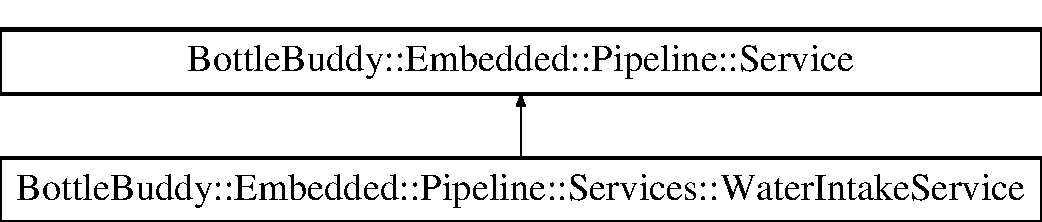
\includegraphics[height=2.000000cm]{class_bottle_buddy_1_1_embedded_1_1_pipeline_1_1_services_1_1_water_intake_service}
\end{center}
\end{figure}
\subsection*{Public Member Functions}
\begin{DoxyCompactItemize}
\item 
{\bfseries Water\+Intake\+Service} (const char $\ast$\hyperlink{class_bottle_buddy_1_1_embedded_1_1_pipeline_1_1_service_af290f9aa0a6dca36e802e615fab19f78}{uid})\hypertarget{class_bottle_buddy_1_1_embedded_1_1_pipeline_1_1_services_1_1_water_intake_service_a0a7366a3c4ea9c7720a5a18129fac62f}{}\label{class_bottle_buddy_1_1_embedded_1_1_pipeline_1_1_services_1_1_water_intake_service_a0a7366a3c4ea9c7720a5a18129fac62f}

\item 
void {\bfseries connect} ()\hypertarget{class_bottle_buddy_1_1_embedded_1_1_pipeline_1_1_services_1_1_water_intake_service_a8eb71ebb9cd53e68847fdc67adc54ae9}{}\label{class_bottle_buddy_1_1_embedded_1_1_pipeline_1_1_services_1_1_water_intake_service_a8eb71ebb9cd53e68847fdc67adc54ae9}

\item 
void {\bfseries disconnect} ()\hypertarget{class_bottle_buddy_1_1_embedded_1_1_pipeline_1_1_services_1_1_water_intake_service_a43c5c1869c79079fcfd8d6b7bdd10821}{}\label{class_bottle_buddy_1_1_embedded_1_1_pipeline_1_1_services_1_1_water_intake_service_a43c5c1869c79079fcfd8d6b7bdd10821}

\item 
void {\bfseries loop} ()\hypertarget{class_bottle_buddy_1_1_embedded_1_1_pipeline_1_1_services_1_1_water_intake_service_adbc1a38d314fb9d071719ebc69fe1a71}{}\label{class_bottle_buddy_1_1_embedded_1_1_pipeline_1_1_services_1_1_water_intake_service_adbc1a38d314fb9d071719ebc69fe1a71}

\item 
void \hyperlink{class_bottle_buddy_1_1_embedded_1_1_pipeline_1_1_services_1_1_water_intake_service_abfa1b38af16fae314c3ba3f80b2bf785}{receive} (\hyperlink{class_bottle_buddy_1_1_embedded_1_1_pipeline_1_1_package}{Package} $\ast$package)
\begin{DoxyCompactList}\small\item\em Used by the router class to deliver a package to a service. \end{DoxyCompactList}\end{DoxyCompactItemize}
\subsection*{Additional Inherited Members}


\subsection{Detailed Description}
This service tracks how much water a Bottle Buddy user drinks throughout the day. 

Specifically, the service creates a set of timestamped values corresponding to when and how much water a user drank during the day. Additionally, it streams this dataset to the Bottle Buddy App. 

\subsection{Member Function Documentation}
\index{Bottle\+Buddy\+::\+Embedded\+::\+Pipeline\+::\+Services\+::\+Water\+Intake\+Service@{Bottle\+Buddy\+::\+Embedded\+::\+Pipeline\+::\+Services\+::\+Water\+Intake\+Service}!receive@{receive}}
\index{receive@{receive}!Bottle\+Buddy\+::\+Embedded\+::\+Pipeline\+::\+Services\+::\+Water\+Intake\+Service@{Bottle\+Buddy\+::\+Embedded\+::\+Pipeline\+::\+Services\+::\+Water\+Intake\+Service}}
\subsubsection[{\texorpdfstring{receive(\+Package $\ast$package)}{receive(Package *package)}}]{\setlength{\rightskip}{0pt plus 5cm}void Bottle\+Buddy\+::\+Embedded\+::\+Pipeline\+::\+Services\+::\+Water\+Intake\+Service\+::receive (
\begin{DoxyParamCaption}
\item[{{\bf Package} $\ast$}]{package}
\end{DoxyParamCaption}
)\hspace{0.3cm}{\ttfamily [virtual]}}\hypertarget{class_bottle_buddy_1_1_embedded_1_1_pipeline_1_1_services_1_1_water_intake_service_abfa1b38af16fae314c3ba3f80b2bf785}{}\label{class_bottle_buddy_1_1_embedded_1_1_pipeline_1_1_services_1_1_water_intake_service_abfa1b38af16fae314c3ba3f80b2bf785}


Used by the router class to deliver a package to a service. 

Can be implemented however the derived service needs in order to provide its service. 

Implements \hyperlink{class_bottle_buddy_1_1_embedded_1_1_pipeline_1_1_service_aaa0ee18450e47f2ad51d9934a2d61992}{Bottle\+Buddy\+::\+Embedded\+::\+Pipeline\+::\+Service}.



The documentation for this class was generated from the following files\+:\begin{DoxyCompactItemize}
\item 
/home/travis/build/\+Bottle\+Buddy/bottle-\/buddy-\/embedded/include/\+Pipeline/\+Services/\hyperlink{water_intake_service_8h}{water\+Intake\+Service.\+h}\item 
/home/travis/build/\+Bottle\+Buddy/bottle-\/buddy-\/embedded/src/\+Pipeline/\+Services/\hyperlink{water_intake_service_8cpp}{water\+Intake\+Service.\+cpp}\end{DoxyCompactItemize}

\hypertarget{struct_bottle_buddy_1_1_embedded_1_1_pipeline_1_1_services_1_1_water_package}{}\section{Bottle\+Buddy\+:\+:Embedded\+:\+:Pipeline\+:\+:Services\+:\+:Water\+Package Struct Reference}
\label{struct_bottle_buddy_1_1_embedded_1_1_pipeline_1_1_services_1_1_water_package}\index{Bottle\+Buddy\+::\+Embedded\+::\+Pipeline\+::\+Services\+::\+Water\+Package@{Bottle\+Buddy\+::\+Embedded\+::\+Pipeline\+::\+Services\+::\+Water\+Package}}
\subsection*{Public Attributes}
\begin{DoxyCompactItemize}
\item 
unsigned short {\bfseries id}\hypertarget{struct_bottle_buddy_1_1_embedded_1_1_pipeline_1_1_services_1_1_water_package_ae73a2f28e310cd2d842b18610f0e8c02}{}\label{struct_bottle_buddy_1_1_embedded_1_1_pipeline_1_1_services_1_1_water_package_ae73a2f28e310cd2d842b18610f0e8c02}

\item 
\hyperlink{struct_bottle_buddy_1_1_embedded_1_1_pipeline_1_1_services_1_1_time}{Time} $\ast$ {\bfseries timestamp}\hypertarget{struct_bottle_buddy_1_1_embedded_1_1_pipeline_1_1_services_1_1_water_package_a2184abfff14e71c5301a4590bb553443}{}\label{struct_bottle_buddy_1_1_embedded_1_1_pipeline_1_1_services_1_1_water_package_a2184abfff14e71c5301a4590bb553443}

\item 
unsigned short {\bfseries old\+Height}\hypertarget{struct_bottle_buddy_1_1_embedded_1_1_pipeline_1_1_services_1_1_water_package_a4a5e2f79dc583245575105370aee3c2a}{}\label{struct_bottle_buddy_1_1_embedded_1_1_pipeline_1_1_services_1_1_water_package_a4a5e2f79dc583245575105370aee3c2a}

\item 
unsigned short {\bfseries new\+Height}\hypertarget{struct_bottle_buddy_1_1_embedded_1_1_pipeline_1_1_services_1_1_water_package_acc73e8c93e6ac9b0247b5a6be0cdedf6}{}\label{struct_bottle_buddy_1_1_embedded_1_1_pipeline_1_1_services_1_1_water_package_acc73e8c93e6ac9b0247b5a6be0cdedf6}

\end{DoxyCompactItemize}


The documentation for this struct was generated from the following file\+:\begin{DoxyCompactItemize}
\item 
/home/travis/build/\+Bottle\+Buddy/bottle-\/buddy-\/embedded/include/\+Pipeline/\+Services/\hyperlink{water_intake_service_8h}{water\+Intake\+Service.\+h}\end{DoxyCompactItemize}

\chapter{File Documentation}
\hypertarget{_b_l_e_8h}{}\section{/home/travis/build/\+Bottle\+Buddy/bottle-\/buddy-\/embedded/include/devices/\+B\+LE.h File Reference}
\label{_b_l_e_8h}\index{/home/travis/build/\+Bottle\+Buddy/bottle-\/buddy-\/embedded/include/devices/\+B\+L\+E.\+h@{/home/travis/build/\+Bottle\+Buddy/bottle-\/buddy-\/embedded/include/devices/\+B\+L\+E.\+h}}
{\ttfamily \#include $<$Arduino\+B\+L\+E.\+h$>$}\\*
\subsection*{Functions}
\begin{DoxyCompactItemize}
\item 
int \hyperlink{_b_l_e_8h_a9deb2d7811a7108862f266acb491ee24}{ble\+\_\+device\+\_\+setup} ()
\begin{DoxyCompactList}\small\item\em Bluetooth Low Energy device setup. \end{DoxyCompactList}\item 
int \hyperlink{_b_l_e_8h_aab988963d6fb81879981baf3ae50f05f}{advertise\+\_\+ble} ()
\begin{DoxyCompactList}\small\item\em Advertise the B\+LE device. \end{DoxyCompactList}\item 
String {\bfseries wait\+\_\+for\+\_\+ble\+\_\+connection} ()\hypertarget{_b_l_e_8h_a233c0db7ddc25d4389167a92881abfab}{}\label{_b_l_e_8h_a233c0db7ddc25d4389167a92881abfab}

\end{DoxyCompactItemize}


\subsection{Detailed Description}
Functions related to the bluetooth low energy device. 

\subsection{Function Documentation}
\index{B\+L\+E.\+h@{B\+L\+E.\+h}!advertise\+\_\+ble@{advertise\+\_\+ble}}
\index{advertise\+\_\+ble@{advertise\+\_\+ble}!B\+L\+E.\+h@{B\+L\+E.\+h}}
\subsubsection[{\texorpdfstring{advertise\+\_\+ble()}{advertise_ble()}}]{\setlength{\rightskip}{0pt plus 5cm}int advertise\+\_\+ble (
\begin{DoxyParamCaption}
{}
\end{DoxyParamCaption}
)}\hypertarget{_b_l_e_8h_aab988963d6fb81879981baf3ae50f05f}{}\label{_b_l_e_8h_aab988963d6fb81879981baf3ae50f05f}


Advertise the B\+LE device. 

Used when ready to advertise B\+LE. \index{B\+L\+E.\+h@{B\+L\+E.\+h}!ble\+\_\+device\+\_\+setup@{ble\+\_\+device\+\_\+setup}}
\index{ble\+\_\+device\+\_\+setup@{ble\+\_\+device\+\_\+setup}!B\+L\+E.\+h@{B\+L\+E.\+h}}
\subsubsection[{\texorpdfstring{ble\+\_\+device\+\_\+setup()}{ble_device_setup()}}]{\setlength{\rightskip}{0pt plus 5cm}int ble\+\_\+device\+\_\+setup (
\begin{DoxyParamCaption}
{}
\end{DoxyParamCaption}
)}\hypertarget{_b_l_e_8h_a9deb2d7811a7108862f266acb491ee24}{}\label{_b_l_e_8h_a9deb2d7811a7108862f266acb491ee24}


Bluetooth Low Energy device setup. 

Call once to set up B\+LE device. 
\hypertarget{_f_s_r_8h}{}\section{/home/travis/build/\+Bottle\+Buddy/bottle-\/buddy-\/embedded/include/devices/\+F\+SR.h File Reference}
\label{_f_s_r_8h}\index{/home/travis/build/\+Bottle\+Buddy/bottle-\/buddy-\/embedded/include/devices/\+F\+S\+R.\+h@{/home/travis/build/\+Bottle\+Buddy/bottle-\/buddy-\/embedded/include/devices/\+F\+S\+R.\+h}}
{\ttfamily \#include $<$Arduino.\+h$>$}\\*
\subsection*{Functions}
\begin{DoxyCompactItemize}
\item 
int {\bfseries read\+\_\+fsr\+\_\+1} ()\hypertarget{_f_s_r_8h_af2bc42c6d12a24ec4fabf0bb4849a77b}{}\label{_f_s_r_8h_af2bc42c6d12a24ec4fabf0bb4849a77b}

\item 
int {\bfseries read\+\_\+fsr\+\_\+2} ()\hypertarget{_f_s_r_8h_aec2bb1f66e483966060b7af611660724}{}\label{_f_s_r_8h_aec2bb1f66e483966060b7af611660724}

\end{DoxyCompactItemize}
\subsection*{Variables}
\begin{DoxyCompactItemize}
\item 
const int {\bfseries fsr\+\_\+pin\+\_\+1}\hypertarget{_f_s_r_8h_ac5f3e6a40904630449137ffc3fb6ac35}{}\label{_f_s_r_8h_ac5f3e6a40904630449137ffc3fb6ac35}

\item 
const int {\bfseries fsr\+\_\+pin\+\_\+2}\hypertarget{_f_s_r_8h_a67ab192b16012c284eeeaea1d70aa6bd}{}\label{_f_s_r_8h_a67ab192b16012c284eeeaea1d70aa6bd}

\end{DoxyCompactItemize}


\subsection{Detailed Description}
Functions related to the force sensitive resistor. 
\hypertarget{_i_m_u_8h}{}\section{/home/travis/build/\+Bottle\+Buddy/bottle-\/buddy-\/embedded/include/devices/\+I\+MU.h File Reference}
\label{_i_m_u_8h}\index{/home/travis/build/\+Bottle\+Buddy/bottle-\/buddy-\/embedded/include/devices/\+I\+M\+U.\+h@{/home/travis/build/\+Bottle\+Buddy/bottle-\/buddy-\/embedded/include/devices/\+I\+M\+U.\+h}}


Functions related to the Inertial Measurement Unit.  


{\ttfamily \#include $<$Arduino\+\_\+\+L\+S\+M9\+D\+S1.\+h$>$}\\*
\subsection*{Functions}
\begin{DoxyCompactItemize}
\item 
int \hyperlink{_i_m_u_8h_a542db9544621cf4d35080293ffde18e8}{imu\+\_\+sensor\+\_\+setup} ()
\begin{DoxyCompactList}\small\item\em Inertial Measurement Unit setup. \end{DoxyCompactList}\item 
void \hyperlink{_i_m_u_8h_ae98c1cd50a46a950918eccac147d188d}{read\+\_\+accelerometer} (float \&x, float \&y, float \&z)
\begin{DoxyCompactList}\small\item\em Grab x, y, and z accelerometer values. \end{DoxyCompactList}\item 
void \hyperlink{_i_m_u_8h_a9c396184b36eea18b681402e2a60f1e5}{read\+\_\+gyroscope} (float \&x, float \&y, float \&z)
\begin{DoxyCompactList}\small\item\em Grab x, y, and z gyroscope values. \end{DoxyCompactList}\item 
void \hyperlink{_i_m_u_8h_ab18d4331cda9888921af1c0b7b32f7a9}{read\+\_\+magnetometer} (float \&x, float \&y, float \&z)
\begin{DoxyCompactList}\small\item\em Grab x, y, and z magnetometer values. \end{DoxyCompactList}\end{DoxyCompactItemize}


\subsection{Detailed Description}
Functions related to the Inertial Measurement Unit. 



\subsection{Function Documentation}
\index{I\+M\+U.\+h@{I\+M\+U.\+h}!imu\+\_\+sensor\+\_\+setup@{imu\+\_\+sensor\+\_\+setup}}
\index{imu\+\_\+sensor\+\_\+setup@{imu\+\_\+sensor\+\_\+setup}!I\+M\+U.\+h@{I\+M\+U.\+h}}
\subsubsection[{\texorpdfstring{imu\+\_\+sensor\+\_\+setup()}{imu_sensor_setup()}}]{\setlength{\rightskip}{0pt plus 5cm}int imu\+\_\+sensor\+\_\+setup (
\begin{DoxyParamCaption}
{}
\end{DoxyParamCaption}
)}\hypertarget{_i_m_u_8h_a542db9544621cf4d35080293ffde18e8}{}\label{_i_m_u_8h_a542db9544621cf4d35080293ffde18e8}


Inertial Measurement Unit setup. 

Call once to set up all three facets of the I\+MU. \index{I\+M\+U.\+h@{I\+M\+U.\+h}!read\+\_\+accelerometer@{read\+\_\+accelerometer}}
\index{read\+\_\+accelerometer@{read\+\_\+accelerometer}!I\+M\+U.\+h@{I\+M\+U.\+h}}
\subsubsection[{\texorpdfstring{read\+\_\+accelerometer(float \&x, float \&y, float \&z)}{read_accelerometer(float &x, float &y, float &z)}}]{\setlength{\rightskip}{0pt plus 5cm}void read\+\_\+accelerometer (
\begin{DoxyParamCaption}
\item[{float \&}]{x, }
\item[{float \&}]{y, }
\item[{float \&}]{z}
\end{DoxyParamCaption}
)}\hypertarget{_i_m_u_8h_ae98c1cd50a46a950918eccac147d188d}{}\label{_i_m_u_8h_ae98c1cd50a46a950918eccac147d188d}


Grab x, y, and z accelerometer values. 

Spins while measurements are not available, then writes accelerometer values to the memory locations specified by parameters. \index{I\+M\+U.\+h@{I\+M\+U.\+h}!read\+\_\+gyroscope@{read\+\_\+gyroscope}}
\index{read\+\_\+gyroscope@{read\+\_\+gyroscope}!I\+M\+U.\+h@{I\+M\+U.\+h}}
\subsubsection[{\texorpdfstring{read\+\_\+gyroscope(float \&x, float \&y, float \&z)}{read_gyroscope(float &x, float &y, float &z)}}]{\setlength{\rightskip}{0pt plus 5cm}void read\+\_\+gyroscope (
\begin{DoxyParamCaption}
\item[{float \&}]{x, }
\item[{float \&}]{y, }
\item[{float \&}]{z}
\end{DoxyParamCaption}
)}\hypertarget{_i_m_u_8h_a9c396184b36eea18b681402e2a60f1e5}{}\label{_i_m_u_8h_a9c396184b36eea18b681402e2a60f1e5}


Grab x, y, and z gyroscope values. 

Spins while measurements are not available, then writes gyroscope values to the memory locations specified by parameters. \index{I\+M\+U.\+h@{I\+M\+U.\+h}!read\+\_\+magnetometer@{read\+\_\+magnetometer}}
\index{read\+\_\+magnetometer@{read\+\_\+magnetometer}!I\+M\+U.\+h@{I\+M\+U.\+h}}
\subsubsection[{\texorpdfstring{read\+\_\+magnetometer(float \&x, float \&y, float \&z)}{read_magnetometer(float &x, float &y, float &z)}}]{\setlength{\rightskip}{0pt plus 5cm}void read\+\_\+magnetometer (
\begin{DoxyParamCaption}
\item[{float \&}]{x, }
\item[{float \&}]{y, }
\item[{float \&}]{z}
\end{DoxyParamCaption}
)}\hypertarget{_i_m_u_8h_ab18d4331cda9888921af1c0b7b32f7a9}{}\label{_i_m_u_8h_ab18d4331cda9888921af1c0b7b32f7a9}


Grab x, y, and z magnetometer values. 

Spins while measurements are not available, then writes magnetometer values to the memory locations specified by parameters. 
\hypertarget{_to_f_8h}{}\section{/home/travis/build/\+Bottle\+Buddy/bottle-\/buddy-\/embedded/include/devices/\+ToF.h File Reference}
\label{_to_f_8h}\index{/home/travis/build/\+Bottle\+Buddy/bottle-\/buddy-\/embedded/include/devices/\+To\+F.\+h@{/home/travis/build/\+Bottle\+Buddy/bottle-\/buddy-\/embedded/include/devices/\+To\+F.\+h}}


Functions related to time of flight sensor.  


{\ttfamily \#include $<$Adafruit\+\_\+\+V\+L53\+L0\+X.\+h$>$}\\*
\subsection*{Functions}
\begin{DoxyCompactItemize}
\item 
int \hyperlink{_to_f_8h_aa3f62fa767072ce3eeb18c5fff68b7d7}{tof\+\_\+sensor\+\_\+setup} ()
\begin{DoxyCompactList}\small\item\em ToF Camera Sensor setup. \end{DoxyCompactList}\item 
int \hyperlink{_to_f_8h_af96f71aa77f1839e156f1e0fd3acefee}{tof\+\_\+sensor\+\_\+distance} ()
\begin{DoxyCompactList}\small\item\em Grab ToF sensor measurement. \end{DoxyCompactList}\end{DoxyCompactItemize}
\subsection*{Variables}
\begin{DoxyCompactItemize}
\item 
const int \hyperlink{_to_f_8h_ae4dbf0330ab067f9cb5f59bcc9caed3e}{B\+A\+U\+D\+\_\+\+R\+A\+TE} = 115200\hypertarget{_to_f_8h_ae4dbf0330ab067f9cb5f59bcc9caed3e}{}\label{_to_f_8h_ae4dbf0330ab067f9cb5f59bcc9caed3e}

\begin{DoxyCompactList}\small\item\em Baud rate. \end{DoxyCompactList}\item 
Adafruit\+\_\+\+V\+L53\+L0X \hyperlink{_to_f_8h_a2ceb0f757748ea460204e32937332e4b}{lox}
\begin{DoxyCompactList}\small\item\em ToF Camera Sensor object. \end{DoxyCompactList}\end{DoxyCompactItemize}


\subsection{Detailed Description}
Functions related to time of flight sensor. 



\subsection{Function Documentation}
\index{To\+F.\+h@{To\+F.\+h}!tof\+\_\+sensor\+\_\+distance@{tof\+\_\+sensor\+\_\+distance}}
\index{tof\+\_\+sensor\+\_\+distance@{tof\+\_\+sensor\+\_\+distance}!To\+F.\+h@{To\+F.\+h}}
\subsubsection[{\texorpdfstring{tof\+\_\+sensor\+\_\+distance()}{tof_sensor_distance()}}]{\setlength{\rightskip}{0pt plus 5cm}int tof\+\_\+sensor\+\_\+distance (
\begin{DoxyParamCaption}
{}
\end{DoxyParamCaption}
)}\hypertarget{_to_f_8h_af96f71aa77f1839e156f1e0fd3acefee}{}\label{_to_f_8h_af96f71aa77f1839e156f1e0fd3acefee}


Grab ToF sensor measurement. 

Can be called continuously to grab the current reading on the ToF sensor. \index{To\+F.\+h@{To\+F.\+h}!tof\+\_\+sensor\+\_\+setup@{tof\+\_\+sensor\+\_\+setup}}
\index{tof\+\_\+sensor\+\_\+setup@{tof\+\_\+sensor\+\_\+setup}!To\+F.\+h@{To\+F.\+h}}
\subsubsection[{\texorpdfstring{tof\+\_\+sensor\+\_\+setup()}{tof_sensor_setup()}}]{\setlength{\rightskip}{0pt plus 5cm}int tof\+\_\+sensor\+\_\+setup (
\begin{DoxyParamCaption}
{}
\end{DoxyParamCaption}
)}\hypertarget{_to_f_8h_aa3f62fa767072ce3eeb18c5fff68b7d7}{}\label{_to_f_8h_aa3f62fa767072ce3eeb18c5fff68b7d7}


ToF Camera Sensor setup. 

Call once to setup the physical sensor. 

\subsection{Variable Documentation}
\index{To\+F.\+h@{To\+F.\+h}!lox@{lox}}
\index{lox@{lox}!To\+F.\+h@{To\+F.\+h}}
\subsubsection[{\texorpdfstring{lox}{lox}}]{\setlength{\rightskip}{0pt plus 5cm}Adafruit\+\_\+\+V\+L53\+L0X lox}\hypertarget{_to_f_8h_a2ceb0f757748ea460204e32937332e4b}{}\label{_to_f_8h_a2ceb0f757748ea460204e32937332e4b}


ToF Camera Sensor object. 

Used to interface with the physical sensor. 
\hypertarget{package_8h}{}\section{/home/travis/build/\+Bottle\+Buddy/bottle-\/buddy-\/embedded/include/\+Pipeline/package.h File Reference}
\label{package_8h}\index{/home/travis/build/\+Bottle\+Buddy/bottle-\/buddy-\/embedded/include/\+Pipeline/package.\+h@{/home/travis/build/\+Bottle\+Buddy/bottle-\/buddy-\/embedded/include/\+Pipeline/package.\+h}}
{\ttfamily \#include $<$stdlib.\+h$>$}\\*
\subsection*{Classes}
\begin{DoxyCompactItemize}
\item 
class \hyperlink{class_bottle_buddy_1_1_embedded_1_1_pipeline_1_1_package}{Bottle\+Buddy\+::\+Embedded\+::\+Pipeline\+::\+Package}
\begin{DoxyCompactList}\small\item\em Encapsulates low level sensor data traveling through the pipeline. \end{DoxyCompactList}\end{DoxyCompactItemize}
\subsection*{Enumerations}
\begin{DoxyCompactItemize}
\item 
enum \hyperlink{package_8h_aea2eca0caf9ed97414998f1a2f404682}{Bottle\+Buddy\+::\+Embedded\+::\+Pipeline\+::\+Location} \{ \\*
{\bfseries ToF}, 
{\bfseries A\+C\+C\+E\+L\+E\+R\+O\+M\+E\+T\+ER}, 
{\bfseries G\+Y\+RO}, 
{\bfseries M\+A\+G\+N\+E\+T\+IC}, 
\\*
{\bfseries F\+SR}
 \}\begin{DoxyCompactList}\small\item\em Location corresponding to a low level sensor. \end{DoxyCompactList}
\end{DoxyCompactItemize}


\subsection{Enumeration Type Documentation}
\index{package.\+h@{package.\+h}!Location@{Location}}
\index{Location@{Location}!package.\+h@{package.\+h}}
\subsubsection[{\texorpdfstring{Location}{Location}}]{\setlength{\rightskip}{0pt plus 5cm}enum {\bf Bottle\+Buddy\+::\+Embedded\+::\+Pipeline\+::\+Location}}\hypertarget{package_8h_file_aea2eca0caf9ed97414998f1a2f404682}{}\label{package_8h_file_aea2eca0caf9ed97414998f1a2f404682}


Location corresponding to a low level sensor. 

Used to mark the location of a pipe so that the router class can know what to do with the data that comes down that pipe. 
\hypertarget{pipe_8h}{}\section{/home/travis/build/\+Bottle\+Buddy/bottle-\/buddy-\/embedded/include/\+Pipeline/pipe.h File Reference}
\label{pipe_8h}\index{/home/travis/build/\+Bottle\+Buddy/bottle-\/buddy-\/embedded/include/\+Pipeline/pipe.\+h@{/home/travis/build/\+Bottle\+Buddy/bottle-\/buddy-\/embedded/include/\+Pipeline/pipe.\+h}}
{\ttfamily \#include $<$stdexcept$>$}\\*
{\ttfamily \#include \char`\"{}Pipeline/router.\+h\char`\"{}}\\*
\subsection*{Classes}
\begin{DoxyCompactItemize}
\item 
class \hyperlink{class_bottle_buddy_1_1_embedded_1_1_pipeline_1_1_pipe}{Bottle\+Buddy\+::\+Embedded\+::\+Pipeline\+::\+Pipe}
\begin{DoxyCompactList}\small\item\em Transports sensor data. \end{DoxyCompactList}\end{DoxyCompactItemize}

\hypertarget{router_8h}{}\section{/home/travis/build/\+Bottle\+Buddy/bottle-\/buddy-\/embedded/include/\+Pipeline/router.h File Reference}
\label{router_8h}\index{/home/travis/build/\+Bottle\+Buddy/bottle-\/buddy-\/embedded/include/\+Pipeline/router.\+h@{/home/travis/build/\+Bottle\+Buddy/bottle-\/buddy-\/embedded/include/\+Pipeline/router.\+h}}
{\ttfamily \#include $<$unordered\+\_\+map$>$}\\*
{\ttfamily \#include $<$functional$>$}\\*
{\ttfamily \#include $<$vector$>$}\\*
{\ttfamily \#include \char`\"{}Pipeline/package.\+h\char`\"{}}\\*
{\ttfamily \#include \char`\"{}Pipeline/service.\+h\char`\"{}}\\*
\subsection*{Classes}
\begin{DoxyCompactItemize}
\item 
class \hyperlink{class_bottle_buddy_1_1_embedded_1_1_pipeline_1_1_router}{Bottle\+Buddy\+::\+Embedded\+::\+Pipeline\+::\+Router}
\begin{DoxyCompactList}\small\item\em Handles package delivery. \end{DoxyCompactList}\end{DoxyCompactItemize}

\hypertarget{service_8h}{}\section{/home/travis/build/\+Bottle\+Buddy/bottle-\/buddy-\/embedded/include/\+Pipeline/service.h File Reference}
\label{service_8h}\index{/home/travis/build/\+Bottle\+Buddy/bottle-\/buddy-\/embedded/include/\+Pipeline/service.\+h@{/home/travis/build/\+Bottle\+Buddy/bottle-\/buddy-\/embedded/include/\+Pipeline/service.\+h}}
{\ttfamily \#include $<$stdlib.\+h$>$}\\*
{\ttfamily \#include $<$string$>$}\\*
{\ttfamily \#include $<$cstring$>$}\\*
{\ttfamily \#include $<$math.\+h$>$}\\*
{\ttfamily \#include $<$unordered\+\_\+map$>$}\\*
{\ttfamily \#include $<$Arduino\+B\+L\+E.\+h$>$}\\*
{\ttfamily \#include \char`\"{}Pipeline/router.\+h\char`\"{}}\\*
\subsection*{Classes}
\begin{DoxyCompactItemize}
\item 
class \hyperlink{class_bottle_buddy_1_1_embedded_1_1_pipeline_1_1_service}{Bottle\+Buddy\+::\+Embedded\+::\+Pipeline\+::\+Service}
\begin{DoxyCompactList}\small\item\em Base class for high level services. \end{DoxyCompactList}\end{DoxyCompactItemize}
\subsection*{Enumerations}
\begin{DoxyCompactItemize}
\item 
enum {\bfseries Bottle\+Type} \{ {\bfseries Z\+A\+N\+E\+\_\+\+Y\+E\+TI}
 \}\hypertarget{service_8h_a415cabbf4f6e7db7460d800b814f644d}{}\label{service_8h_a415cabbf4f6e7db7460d800b814f644d}

\item 
enum {\bfseries B\+L\+E\+Type} \{ \\*
{\bfseries Unsigned\+Int}, 
{\bfseries Unsigned\+Short}, 
{\bfseries Unsigned\+Char}, 
{\bfseries String}, 
\\*
{\bfseries Boolean}
 \}\hypertarget{service_8h_a7dcc4df0950cda10afaa8e051a8f5436}{}\label{service_8h_a7dcc4df0950cda10afaa8e051a8f5436}

\end{DoxyCompactItemize}

\hypertarget{service_manager_8h}{}\section{/home/travis/build/\+Bottle\+Buddy/bottle-\/buddy-\/embedded/include/\+Pipeline/service\+Manager.h File Reference}
\label{service_manager_8h}\index{/home/travis/build/\+Bottle\+Buddy/bottle-\/buddy-\/embedded/include/\+Pipeline/service\+Manager.\+h@{/home/travis/build/\+Bottle\+Buddy/bottle-\/buddy-\/embedded/include/\+Pipeline/service\+Manager.\+h}}
{\ttfamily \#include $<$vector$>$}\\*
{\ttfamily \#include \char`\"{}Pipeline/\+Services/cleaning\+Service.\+h\char`\"{}}\\*
{\ttfamily \#include \char`\"{}Pipeline/\+Services/water\+Intake\+Service.\+h\char`\"{}}\\*
\subsection*{Classes}
\begin{DoxyCompactItemize}
\item 
class \hyperlink{class_bottle_buddy_1_1_embedded_1_1_pipeline_1_1_service_manager}{Bottle\+Buddy\+::\+Embedded\+::\+Pipeline\+::\+Service\+Manager}
\begin{DoxyCompactList}\small\item\em Manages all instantiated services. \end{DoxyCompactList}\end{DoxyCompactItemize}

\hypertarget{calibration_service_8h}{}\section{/home/travis/build/\+Bottle\+Buddy/bottle-\/buddy-\/embedded/include/\+Pipeline/\+Services/calibration\+Service.h File Reference}
\label{calibration_service_8h}\index{/home/travis/build/\+Bottle\+Buddy/bottle-\/buddy-\/embedded/include/\+Pipeline/\+Services/calibration\+Service.\+h@{/home/travis/build/\+Bottle\+Buddy/bottle-\/buddy-\/embedded/include/\+Pipeline/\+Services/calibration\+Service.\+h}}
{\ttfamily \#include \char`\"{}Pipeline/service.\+h\char`\"{}}\\*
\subsection*{Classes}
\begin{DoxyCompactItemize}
\item 
class \hyperlink{class_bottle_buddy_1_1_embedded_1_1_pipeline_1_1_services_1_1_calibration_service}{Bottle\+Buddy\+::\+Embedded\+::\+Pipeline\+::\+Services\+::\+Calibration\+Service}
\end{DoxyCompactItemize}

\hypertarget{cleaning_service_8h}{}\section{/home/travis/build/\+Bottle\+Buddy/bottle-\/buddy-\/embedded/include/\+Pipeline/\+Services/cleaning\+Service.h File Reference}
\label{cleaning_service_8h}\index{/home/travis/build/\+Bottle\+Buddy/bottle-\/buddy-\/embedded/include/\+Pipeline/\+Services/cleaning\+Service.\+h@{/home/travis/build/\+Bottle\+Buddy/bottle-\/buddy-\/embedded/include/\+Pipeline/\+Services/cleaning\+Service.\+h}}
{\ttfamily \#include $<$arduino-\/timer.\+h$>$}\\*
{\ttfamily \#include \char`\"{}Pipeline/service.\+h\char`\"{}}\\*
\subsection*{Classes}
\begin{DoxyCompactItemize}
\item 
class \hyperlink{class_bottle_buddy_1_1_embedded_1_1_pipeline_1_1_services_1_1_cleaning_service}{Bottle\+Buddy\+::\+Embedded\+::\+Pipeline\+::\+Services\+::\+Cleaning\+Service}
\begin{DoxyCompactList}\small\item\em This class automatically cleans the users bottle. \end{DoxyCompactList}\end{DoxyCompactItemize}

\hypertarget{water_intake_service_8h}{}\section{/home/travis/build/\+Bottle\+Buddy/bottle-\/buddy-\/embedded/include/\+Pipeline/\+Services/water\+Intake\+Service.h File Reference}
\label{water_intake_service_8h}\index{/home/travis/build/\+Bottle\+Buddy/bottle-\/buddy-\/embedded/include/\+Pipeline/\+Services/water\+Intake\+Service.\+h@{/home/travis/build/\+Bottle\+Buddy/bottle-\/buddy-\/embedded/include/\+Pipeline/\+Services/water\+Intake\+Service.\+h}}
{\ttfamily \#include \char`\"{}Pipeline/service.\+h\char`\"{}}\\*
\subsection*{Classes}
\begin{DoxyCompactItemize}
\item 
class \hyperlink{class_bottle_buddy_1_1_embedded_1_1_pipeline_1_1_services_1_1_water_intake_service}{Bottle\+Buddy\+::\+Embedded\+::\+Pipeline\+::\+Services\+::\+Water\+Intake\+Service}
\begin{DoxyCompactList}\small\item\em This service tracks how much water a Bottle Buddy user drinks throughout the day. \end{DoxyCompactList}\end{DoxyCompactItemize}

\hypertarget{main_8cpp}{}\section{/home/travis/build/\+Bottle\+Buddy/bottle-\/buddy-\/embedded/src/main.cpp File Reference}
\label{main_8cpp}\index{/home/travis/build/\+Bottle\+Buddy/bottle-\/buddy-\/embedded/src/main.\+cpp@{/home/travis/build/\+Bottle\+Buddy/bottle-\/buddy-\/embedded/src/main.\+cpp}}


Main file.  


{\ttfamily \#include $<$Arduino.\+h$>$}\\*
\subsection*{Functions}
\begin{DoxyCompactItemize}
\item 
void \hyperlink{main_8cpp_a4fc01d736fe50cf5b977f755b675f11d}{setup} ()
\begin{DoxyCompactList}\small\item\em Setup loop. \end{DoxyCompactList}\item 
void \hyperlink{main_8cpp_afe461d27b9c48d5921c00d521181f12f}{loop} ()
\begin{DoxyCompactList}\small\item\em Main loop. \end{DoxyCompactList}\end{DoxyCompactItemize}
\subsection*{Variables}
\begin{DoxyCompactItemize}
\item 
constexpr int \hyperlink{main_8cpp_afbff995684d75e5a671be4c1afa783e8}{serial\+Speed} = 115200\hypertarget{main_8cpp_afbff995684d75e5a671be4c1afa783e8}{}\label{main_8cpp_afbff995684d75e5a671be4c1afa783e8}

\begin{DoxyCompactList}\small\item\em Serial speed. \end{DoxyCompactList}\item 
constexpr int \hyperlink{main_8cpp_ae648b3d2230eb5ca63fac8ee24fd6d76}{delay\+Time} = 1000\hypertarget{main_8cpp_ae648b3d2230eb5ca63fac8ee24fd6d76}{}\label{main_8cpp_ae648b3d2230eb5ca63fac8ee24fd6d76}

\begin{DoxyCompactList}\small\item\em Delay time. \end{DoxyCompactList}\item 
constexpr int {\bfseries led\+Pin} = 2\hypertarget{main_8cpp_aec84357ffcb51a347174132f17b8a5f5}{}\label{main_8cpp_aec84357ffcb51a347174132f17b8a5f5}

\end{DoxyCompactItemize}


\subsection{Detailed Description}
Main file. 

Entrance point to system. 

\subsection{Function Documentation}
\index{main.\+cpp@{main.\+cpp}!loop@{loop}}
\index{loop@{loop}!main.\+cpp@{main.\+cpp}}
\subsubsection[{\texorpdfstring{loop()}{loop()}}]{\setlength{\rightskip}{0pt plus 5cm}void loop (
\begin{DoxyParamCaption}
{}
\end{DoxyParamCaption}
)}\hypertarget{main_8cpp_afe461d27b9c48d5921c00d521181f12f}{}\label{main_8cpp_afe461d27b9c48d5921c00d521181f12f}


Main loop. 

This loop blinks an L\+ED for demonstration purposes. \index{main.\+cpp@{main.\+cpp}!setup@{setup}}
\index{setup@{setup}!main.\+cpp@{main.\+cpp}}
\subsubsection[{\texorpdfstring{setup()}{setup()}}]{\setlength{\rightskip}{0pt plus 5cm}void setup (
\begin{DoxyParamCaption}
{}
\end{DoxyParamCaption}
)}\hypertarget{main_8cpp_a4fc01d736fe50cf5b977f755b675f11d}{}\label{main_8cpp_a4fc01d736fe50cf5b977f755b675f11d}


Setup loop. 

Makes necessary initializations for system to be able to run. 
\hypertarget{package_8cpp}{}\section{/home/travis/build/\+Bottle\+Buddy/bottle-\/buddy-\/embedded/src/\+Pipeline/package.cpp File Reference}
\label{package_8cpp}\index{/home/travis/build/\+Bottle\+Buddy/bottle-\/buddy-\/embedded/src/\+Pipeline/package.\+cpp@{/home/travis/build/\+Bottle\+Buddy/bottle-\/buddy-\/embedded/src/\+Pipeline/package.\+cpp}}
{\ttfamily \#include \char`\"{}Pipeline/package.\+h\char`\"{}}\\*

\hypertarget{pipe_8cpp}{}\section{/home/travis/build/\+Bottle\+Buddy/bottle-\/buddy-\/embedded/src/\+Pipeline/pipe.cpp File Reference}
\label{pipe_8cpp}\index{/home/travis/build/\+Bottle\+Buddy/bottle-\/buddy-\/embedded/src/\+Pipeline/pipe.\+cpp@{/home/travis/build/\+Bottle\+Buddy/bottle-\/buddy-\/embedded/src/\+Pipeline/pipe.\+cpp}}
{\ttfamily \#include \char`\"{}Pipeline/pipe.\+h\char`\"{}}\\*

\hypertarget{router_8cpp}{}\section{/home/travis/build/\+Bottle\+Buddy/bottle-\/buddy-\/embedded/src/\+Pipeline/router.cpp File Reference}
\label{router_8cpp}\index{/home/travis/build/\+Bottle\+Buddy/bottle-\/buddy-\/embedded/src/\+Pipeline/router.\+cpp@{/home/travis/build/\+Bottle\+Buddy/bottle-\/buddy-\/embedded/src/\+Pipeline/router.\+cpp}}
{\ttfamily \#include \char`\"{}Pipeline/router.\+h\char`\"{}}\\*

\hypertarget{service_8cpp}{}\section{/home/travis/build/\+Bottle\+Buddy/bottle-\/buddy-\/embedded/src/\+Pipeline/service.cpp File Reference}
\label{service_8cpp}\index{/home/travis/build/\+Bottle\+Buddy/bottle-\/buddy-\/embedded/src/\+Pipeline/service.\+cpp@{/home/travis/build/\+Bottle\+Buddy/bottle-\/buddy-\/embedded/src/\+Pipeline/service.\+cpp}}
{\ttfamily \#include \char`\"{}Pipeline/service.\+h\char`\"{}}\\*

\hypertarget{service_manager_8cpp}{}\section{/home/travis/build/\+Bottle\+Buddy/bottle-\/buddy-\/embedded/src/\+Pipeline/service\+Manager.cpp File Reference}
\label{service_manager_8cpp}\index{/home/travis/build/\+Bottle\+Buddy/bottle-\/buddy-\/embedded/src/\+Pipeline/service\+Manager.\+cpp@{/home/travis/build/\+Bottle\+Buddy/bottle-\/buddy-\/embedded/src/\+Pipeline/service\+Manager.\+cpp}}
{\ttfamily \#include \char`\"{}Pipeline/service\+Manager.\+h\char`\"{}}\\*

\hypertarget{calibration_service_8cpp}{}\section{/home/travis/build/\+Bottle\+Buddy/bottle-\/buddy-\/embedded/src/\+Pipeline/\+Services/calibration\+Service.cpp File Reference}
\label{calibration_service_8cpp}\index{/home/travis/build/\+Bottle\+Buddy/bottle-\/buddy-\/embedded/src/\+Pipeline/\+Services/calibration\+Service.\+cpp@{/home/travis/build/\+Bottle\+Buddy/bottle-\/buddy-\/embedded/src/\+Pipeline/\+Services/calibration\+Service.\+cpp}}
{\ttfamily \#include \char`\"{}Pipeline/\+Services/calibration\+Service.\+h\char`\"{}}\\*

\hypertarget{cleaning_service_8cpp}{}\section{/home/travis/build/\+Bottle\+Buddy/bottle-\/buddy-\/embedded/src/\+Pipeline/\+Services/cleaning\+Service.cpp File Reference}
\label{cleaning_service_8cpp}\index{/home/travis/build/\+Bottle\+Buddy/bottle-\/buddy-\/embedded/src/\+Pipeline/\+Services/cleaning\+Service.\+cpp@{/home/travis/build/\+Bottle\+Buddy/bottle-\/buddy-\/embedded/src/\+Pipeline/\+Services/cleaning\+Service.\+cpp}}
{\ttfamily \#include \char`\"{}Pipeline/\+Services/cleaning\+Service.\+h\char`\"{}}\\*

\hypertarget{water_intake_service_8cpp}{}\section{/home/travis/build/\+Bottle\+Buddy/bottle-\/buddy-\/embedded/src/\+Pipeline/\+Services/water\+Intake\+Service.cpp File Reference}
\label{water_intake_service_8cpp}\index{/home/travis/build/\+Bottle\+Buddy/bottle-\/buddy-\/embedded/src/\+Pipeline/\+Services/water\+Intake\+Service.\+cpp@{/home/travis/build/\+Bottle\+Buddy/bottle-\/buddy-\/embedded/src/\+Pipeline/\+Services/water\+Intake\+Service.\+cpp}}
{\ttfamily \#include \char`\"{}Pipeline/\+Services/water\+Intake\+Service.\+h\char`\"{}}\\*

%--- End generated contents ---

% Index
\backmatter
\newpage
\phantomsection
\clearemptydoublepage
\addcontentsline{toc}{chapter}{Index}
\printindex

\end{document}
